\chapter{Koncept funkčnosti testeru}
Tato kapitola definuje rozsah diplomové práce a podává úvodní náhled na funkčnost navrhovaných zařízení.

\section{Princip funkčnosti ICT testeru}

    ICT tester se skládá ze dvou hlavních částí \mbox{(měřící a fixture).}
    Měřící část obsahuje různé měřící přístroje např.
    osciloskop, multimeter, proudové a napěťové zdroje, boundary scan atd.
    Pomocí těchto zařízení ICT tester provádí různá měření.\\

    Fixture je vyměnitelnou částí a obsahuje zakládací pole s testovacími jehlami (Probes).
    Testovací jehly zajišťují elektrické propojení mezi testovanými body na PCB a měřící částí.
    Ze spodní strany je fixture propojena s měřící částí pomocí matice bRC pinů.
    Písmena R a C v označení bRC označují Row (řádek) a Column (sloupec).\\

    Fixture umožňuje mezi sebou libovolně propojovat bRC a Probes piny, včetně propojení pinů stejného druhu mezi sebou.
    Propojení mezi jednotlivými piny je většinou zajištěno pomocí ovíjení. Nicméně propojení může obsahovat i různé pasivní součástky.
    Obrázek \ref{fig:ICT_tester} znázorňuje jednotlivé části ICT testeru\cite{ICTkeysight}\cite{ICT_picture}.

\begin{figure}[ht]
\centering
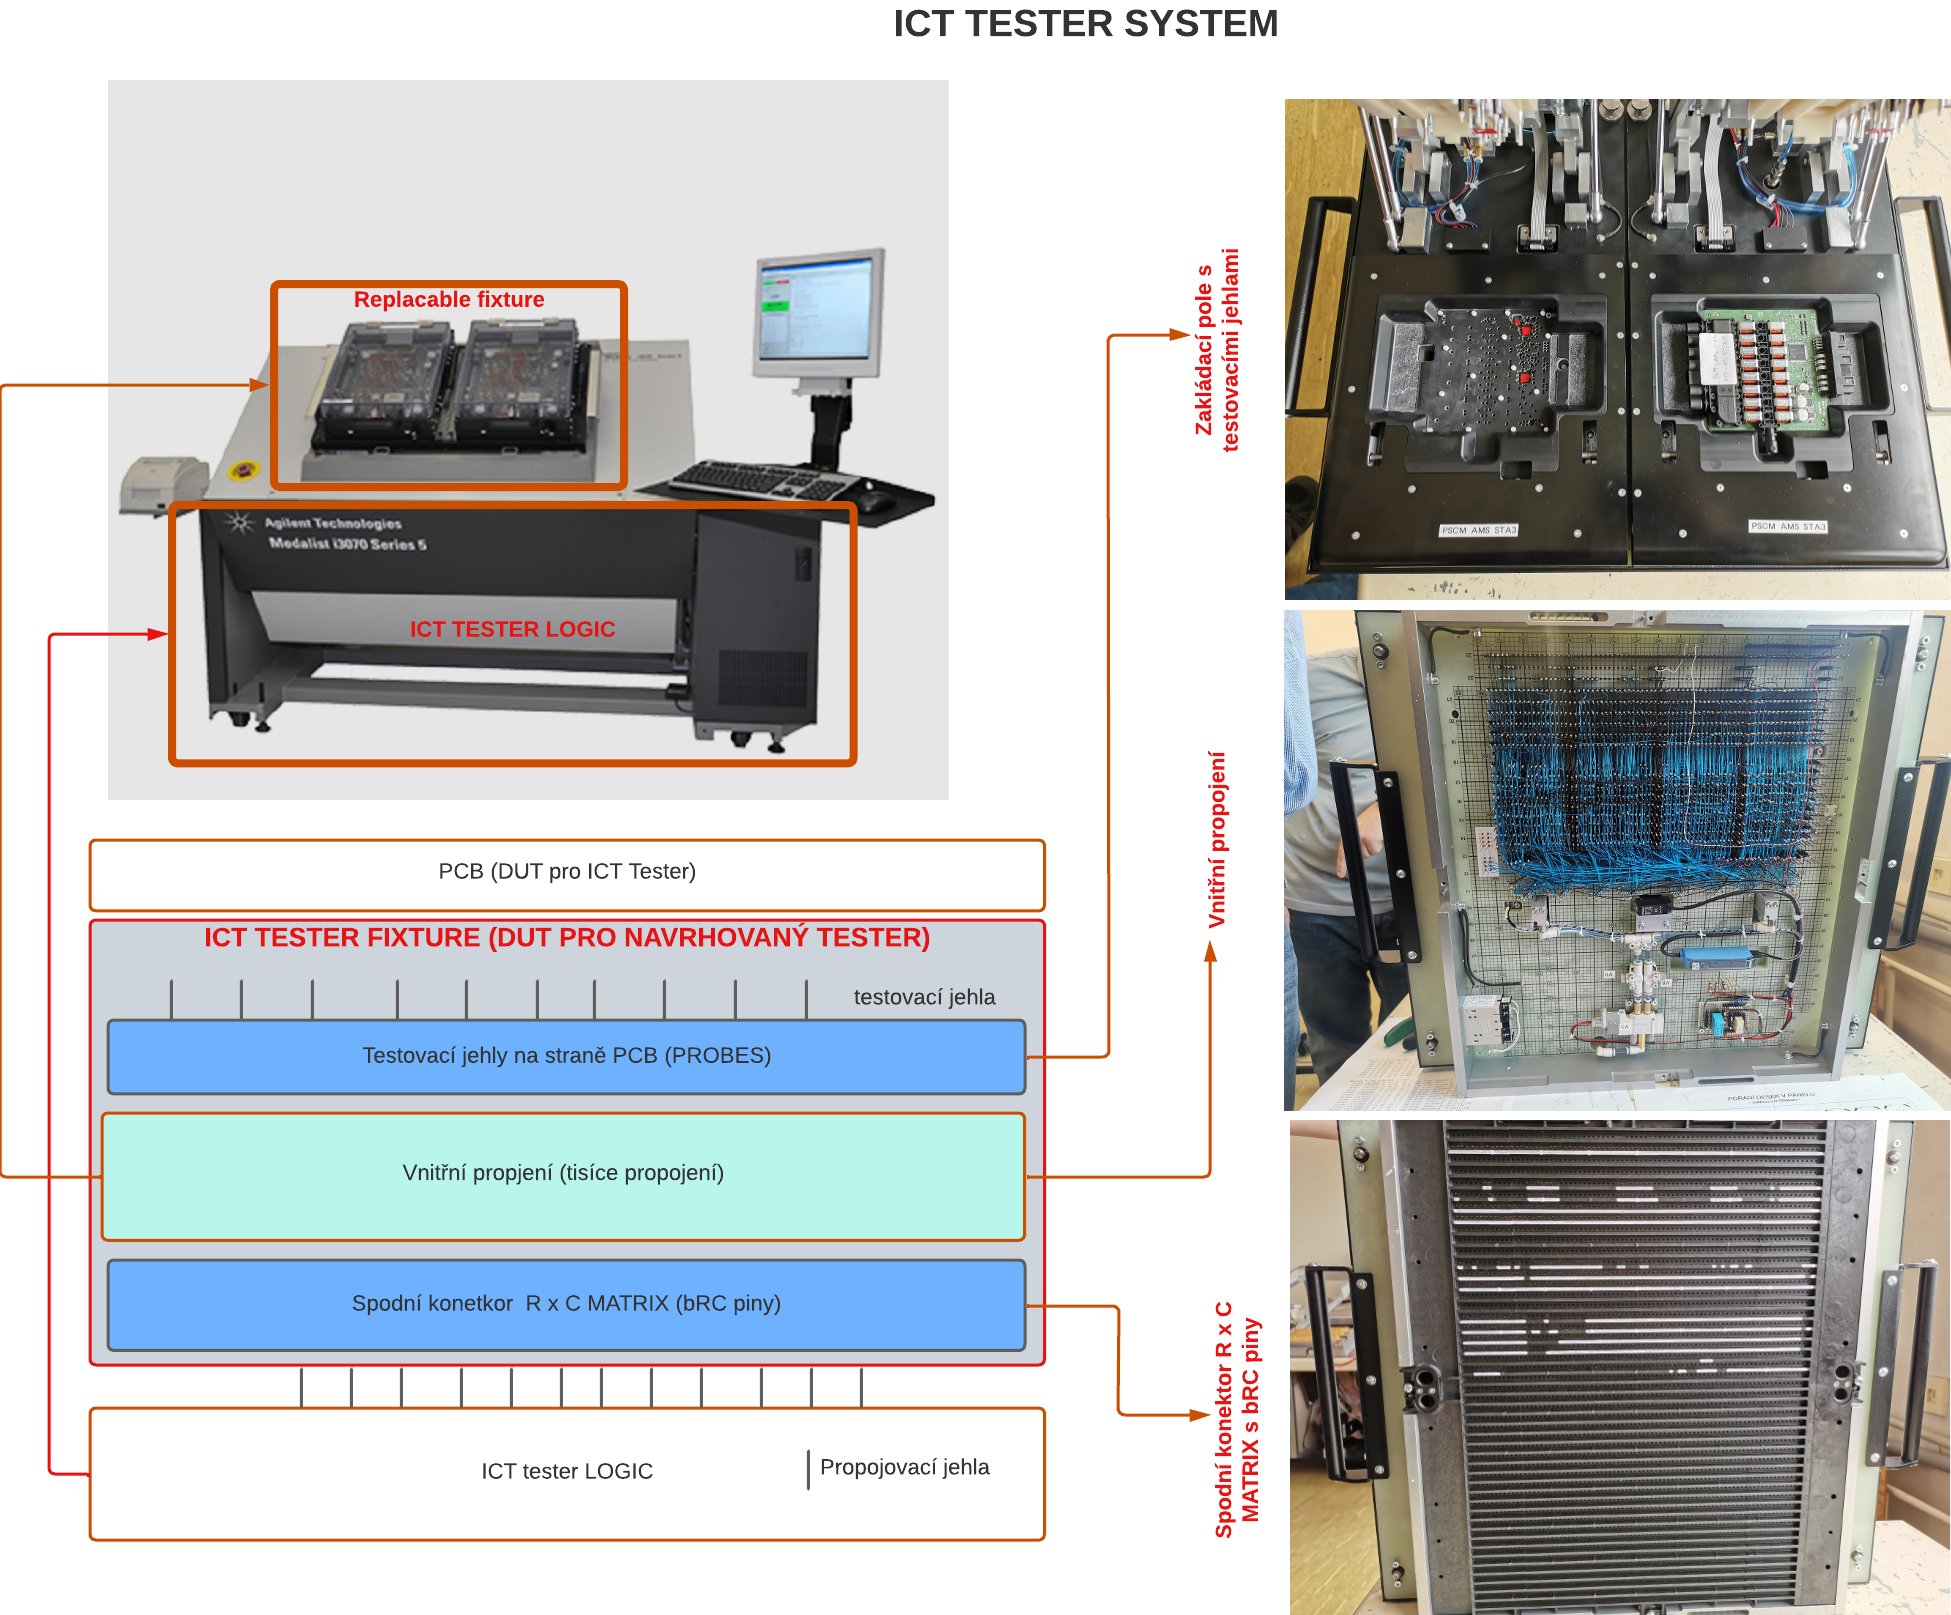
\includegraphics[width=0.9\textwidth]{obrazky/ICT_tester.png}
\caption{Části ICT testeru (obrázek testeru vlevo nahoře převzat z \cite{ICT_picture})}
\label{fig:ICT_tester}
\end{figure}
\clearpage

\section{Koncepce navrhovaného testeru}
Zatímco pro ICT tester bylo úkolem otestovat vložené PCB. Úkolem zařízení, navrhovaným v diplomové práci, je otestovat správnost propojení
fixture části ICT testeru. Pro tento účel je navržena následující koncepce.
\begin{figure}[ht!]
        \centering
        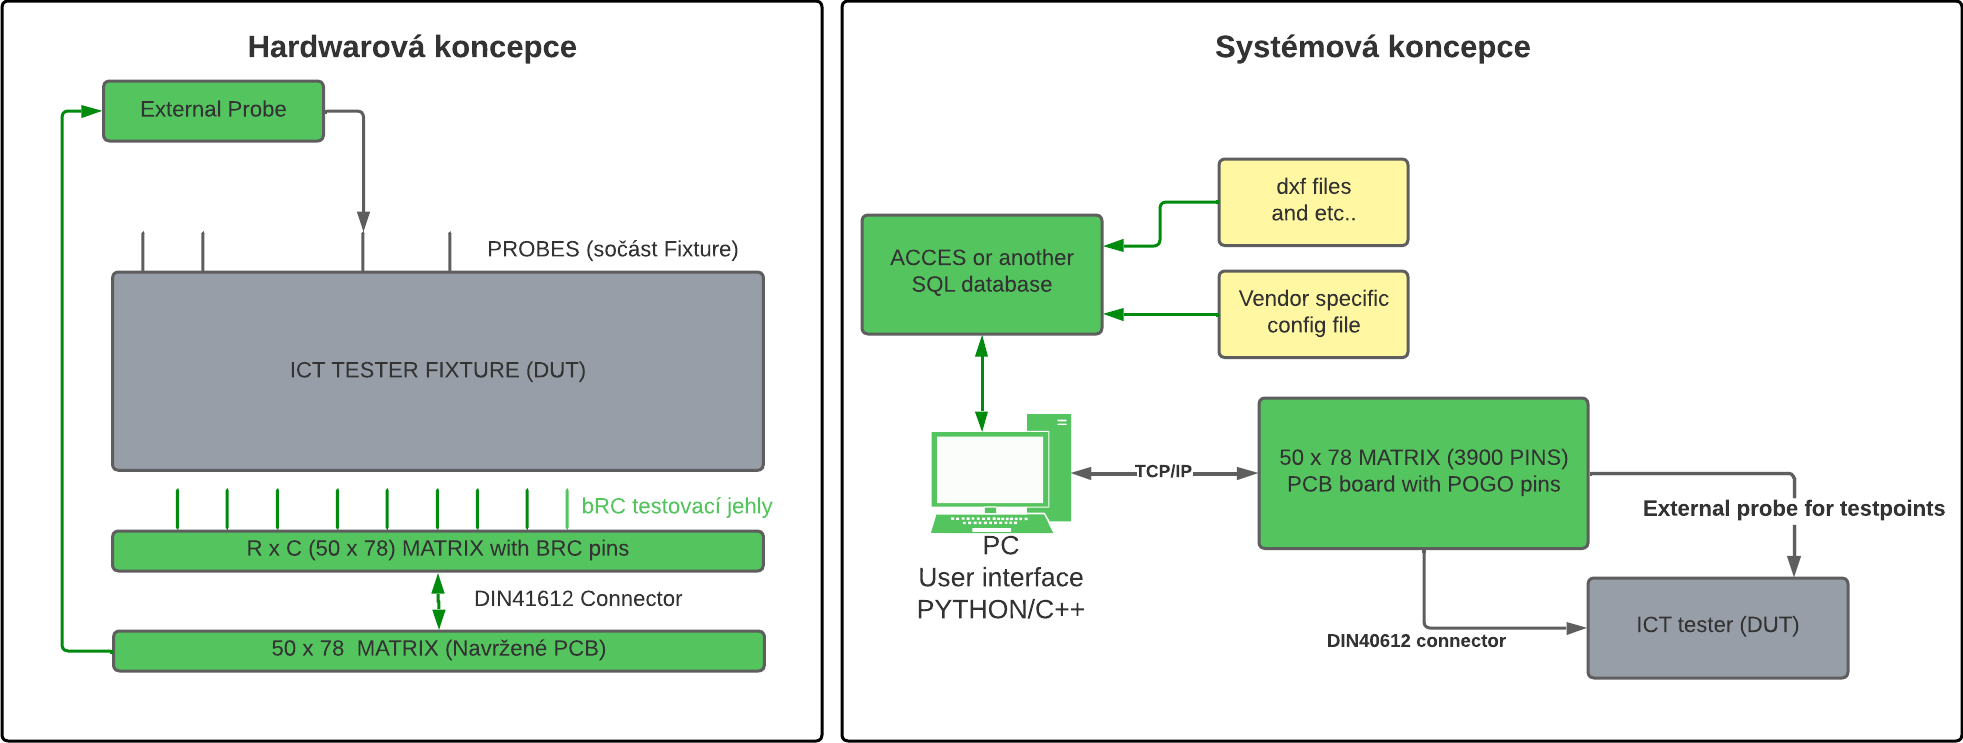
\includegraphics[width = 1\textwidth]{obrazky/system_connection_and_fixture.png}
        \caption{Koncepce funkčnosti navrhovaného testeru}
        \label{fig:Koncepce funkce}
    \end{figure}

    Na obrázku \ref{fig:Koncepce funkce} jsou zeleně znázorněny části, která jsou součástí diplomové práce.
    Ostatní barvy značí části, které již existují a nebudou navrhovány.
    \subsection{Systémová koncepce}
    Na obrázku \ref{fig:Koncepce funkce} v pravé části je znázorněná systémová koncepce testeru.
    Pro otestování vnitřního propojení fixture je nutné propojit všechny bRC piny s logikou navrhovaného testeru.
    Většina komerčních ICT testerů omezuje počet sloupců v bRC MATRIX na 78 a liší se tak pouze počtem řad.
    Z tohoto důvodu je tester navržen tak, aby bylo možné libovolně  měnit počet řad o 78 pinech\cite{ICT_guidline}.\\
    
    \begin{figure}[ht!]
        \centering
        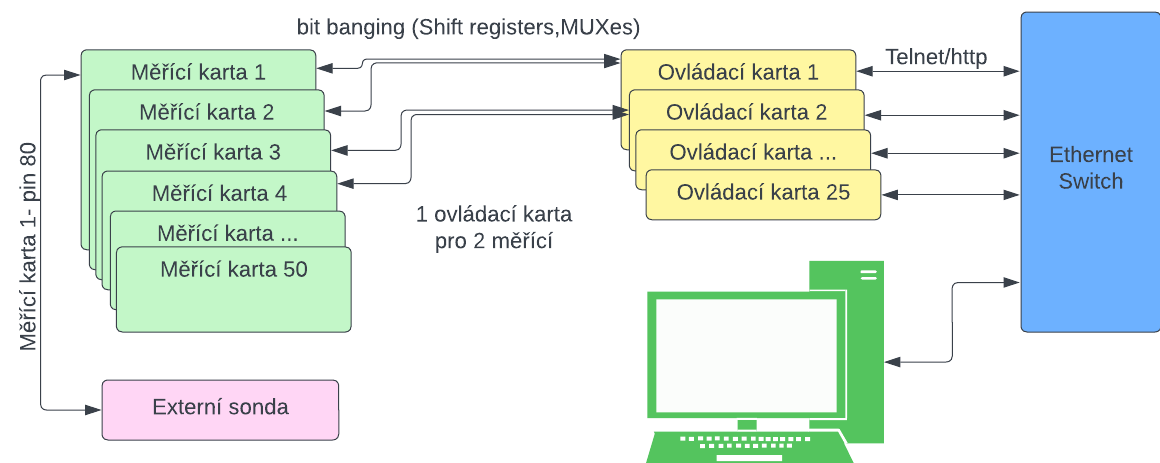
\includegraphics[width = 1\textwidth]{obrazky/telnet_http_pc.png}
        \caption{Systémová koncepce}
        \label{fig:Systémová koncepce}
    \end{figure}

    Navržené zařízení se skládá z měřících karet, ovládacích karet a řídícího počítače
    \mbox{(Obr. \ref{fig:Systémová koncepce})}.
    Úkolem měřící karty je měřit hodnoty odporu mezi jednotlivými bRC piny
    a odesílat data do ovládací karty. Měřící karty jsou kompatibilní s 5V a 3V3 logikou.\\

    \begin{figure}[ht!] 
        \centering
        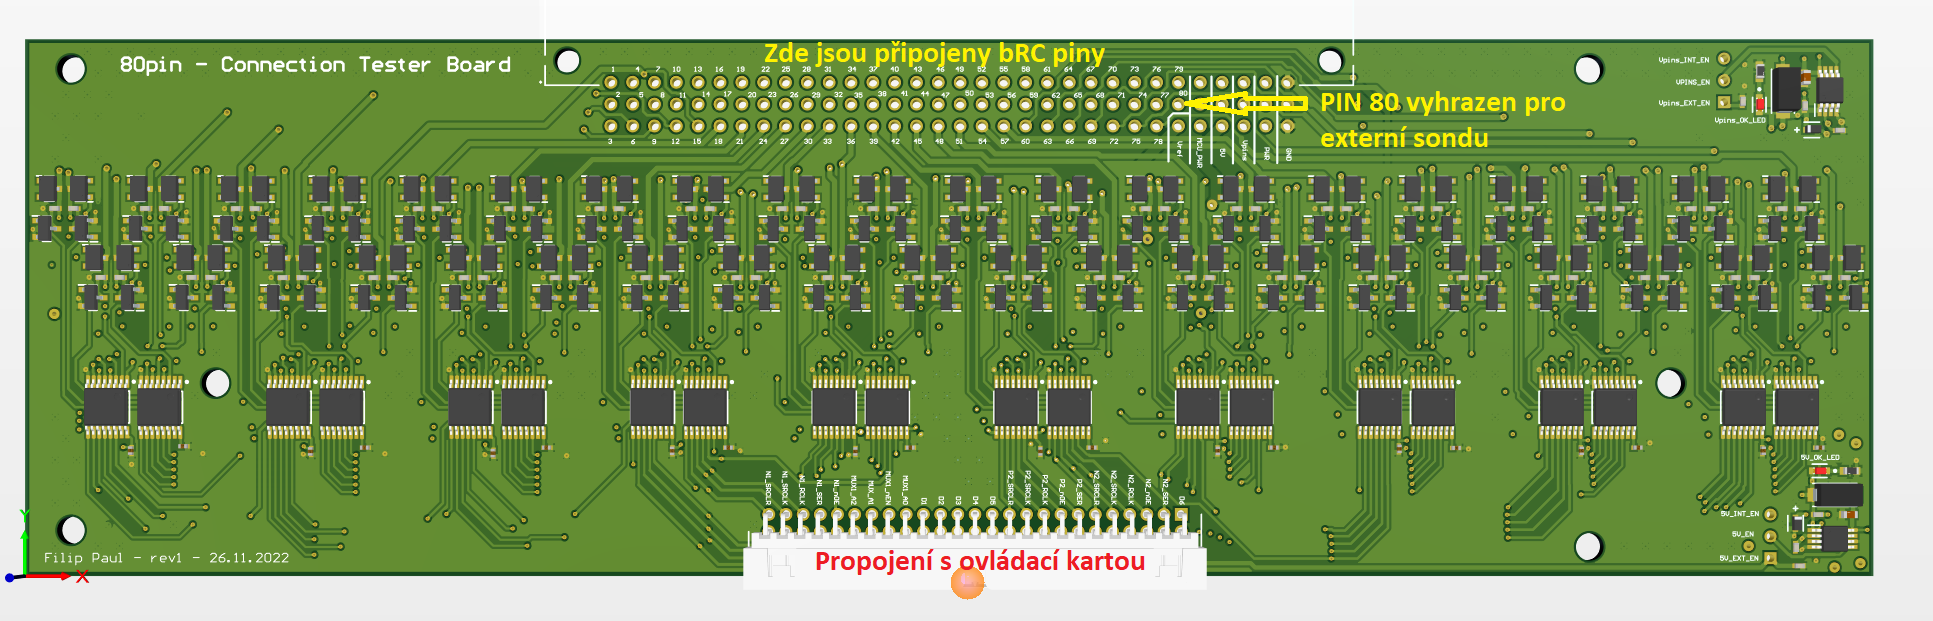
\includegraphics[width = 0.95\textwidth]{obrazky/karta_3D_NP.png}
        \caption{Měřící karta}
        \label{fig:Měřící karta}
    \end{figure}


    \begin{figure}[ht!]
        \centering
        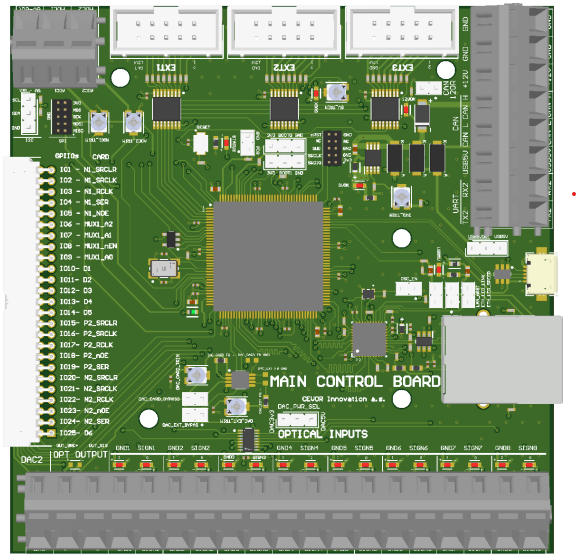
\includegraphics[width = 0.7\textwidth]{obrazky/3D_ovl_karta.png}
        \caption{Ovládací karta - 3D model (Není vyrobena jedná se o předběžný návrh)}
        \label{fig:Ovládací karta - 3D model}
    \end{figure}

    Jednotlivé ovládací karty mají možnost připojení k ethernetové síti pomocí
    100BASE-T PHY a jsou schopny ovládat měřící karty.
    Ovládací karty komunikují pouze s řídící PC aplikací (nikoliv mezi sebou).
    Řídící PC aplikace řídí všechny testy. Ovládací karty mají v sobě implementován Telnet a http server,
    přičemž se pro hlavní komunikaci používá právě Telnet server.
    Takto lze využít jakékoliv zařízení s přístupem do sítě pro řízení testeru.\\
    
    Řídící aplikace využívá ke své činnosti celou řadu vstupních souborů. Jedná se o soubory, které definují zapojení fixture, CAD, CAM a další data\cite{CAD_wiki}.
    Protože vstupní soubory nemají jednotný formát pro každého výrobce, aplikace nejprve data převede do mySQL databáze. S takto zpracovanými daty již lze
    provádět jednotné operace. Aplikace porovnává naměřená data z jednotlivých karet ze vstupními soubory a následně generuje výsledek testu propojení
    v co nejsrozumitelnější podobě.

    \subsection{Hardwarová koncepce}
    \subsubsection{Propojení bRC pinů mezi sebou}

    Propojení mezi měřícími kartami a maticí bRC pinů je zajištěno pomocí POGO pinů (strana fixture),
    bRC jehel (strana testeru) a pneumatického kontaktování.
    Na Obr. \ref{fig:Měřící karta} je znázorněn 3D model měřící karty. V horní části jsou připraveny 
    body pro připojení bRC jehel a napájení desky. Rozteč kontaktů je zvolena tak, aby bylo možno
    k měřící kartě připájet standardizovaný DIN41612 konektor (dále pouze DIN) a kartu tak snadno použít pro jiné aplikace.\\

    Ve spodní části se nachází 25x2 konektor, sloužící k propojení s ovládací kartou. Měřící karta je navržena tak, aby buď poskytovala
    napájení ovládací kartě a nebo byla ovládací kartou napájena (více v sekci o návrhu měřící karty).

    \subsubsection{Propojení mezi bRC a Probes}
    Pomocí karet je možné automaticky zjistit propojení mezi všemi bRC piny,
    nicméně přímé propojení mezi bRC a Probe piny je nutné otestovat zvlášť.
    Za tímto účelem je k testeru připojena externí sonda (Obr. \ref{fig:Systémová koncepce}).
    Sonda je připojena do bRC pinu \hbox{č. 80} na měřící
    kartě \hbox{č. 1.}\\

    Obsluha v závislosti na pokynech PC aplikace připojuje sondu k jednotlivým probes pinům.
    Takto lze pomocí jednotlivých karet zjistit propojení.
    Externí sonda je podobná jako sonda multimetru a slouží pouze k přivedení testovacího napětí na probe pin.
    Proces lze celý automatizovat v případě, že je k dispozici i maketa PCB,
    která bude obsahovat všechny probe piny přivedené na DIN konektor.
    V takovém případě lze připojit maketu PCB k kartě a proces automatizovat.

    \chapter{Návrh měřících karet}
    Tato kapitola se zabývá hardwarovým řešením měřících karet. Dále je zde popsána funkčnost základních bloků karet, výběr komponentů a návrh PCB.

    \section{Základní požadavky na měřící karty}
    Následující seznam popisuje základní požadavky na měřící karty, seznam je seřazen podle priorit.
    \begin{enumerate}
        \item Schopnost měřit odpor mezi jakýmikoliv dvěma bRC piny a to i v případě, že se každý z pinů nachází na jiné kartě.
        \item Komunikace s ovládací kartou.
        \item Škálovatelnost.
        \item Modularitou se rozumí, co největší nezávislost jednotlivých funkčních bloků na sobě.
        \item Dostupnost komponentů. 
        \item Cena komponentů. 
    \end{enumerate}

    \section{Funkční bloky}
    Na následujícím obrázku je znázorněn blokový diagram měřících karet.
    \begin{figure}[ht!]
            \centering
            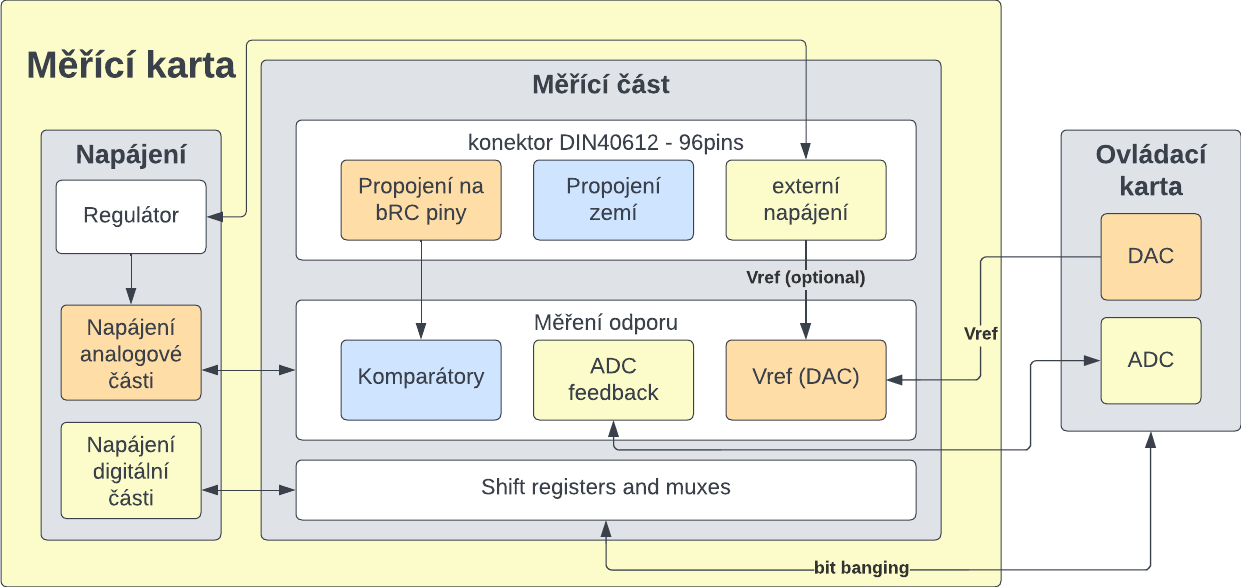
\includegraphics[width = 1\textwidth]{obrazky/karta_system_diagram.png}
            \caption{Blokový diagram měřících karet}
            \label{fig:Blokový diagram měřících karet}
    \end{figure}

        Karta se skládá ze 2 hlavních bloků (Měřící části a napájení). V následujících kapitolách jsou tyto bloky
        podrobně popsány.
        \clearpage

        \subsection{Měřící část}
        \subsubsection{Teoretický návrh}
        Měřící část je zodpovědná za měření odporu mezi dvěma bRC piny.
        Obr. \ref{fig:Napěťový dělič pro 2 a 4 propojené bRC piny} v levé části zobrazuje
        jednoduchý ideální napěťový dělič.
        Dělič je zapojen tak, že jeden z testovaných pinů bRC1 generuje napětí $V_{in}$
        a na druhém pinu bRC2 se měří napětí $V_{out}$.
        Měřeným odporem je odpor Rpath, který lze dopočítat následovně:\\
        
        \begin{equation}\label{eq:odpor delic}
            R_{path} = \frac{(V_{in} - V_{out}) \cdot R_x}{V_{out}}
        \end{equation}
        
    \begin{figure}[ht!]
            \centering
            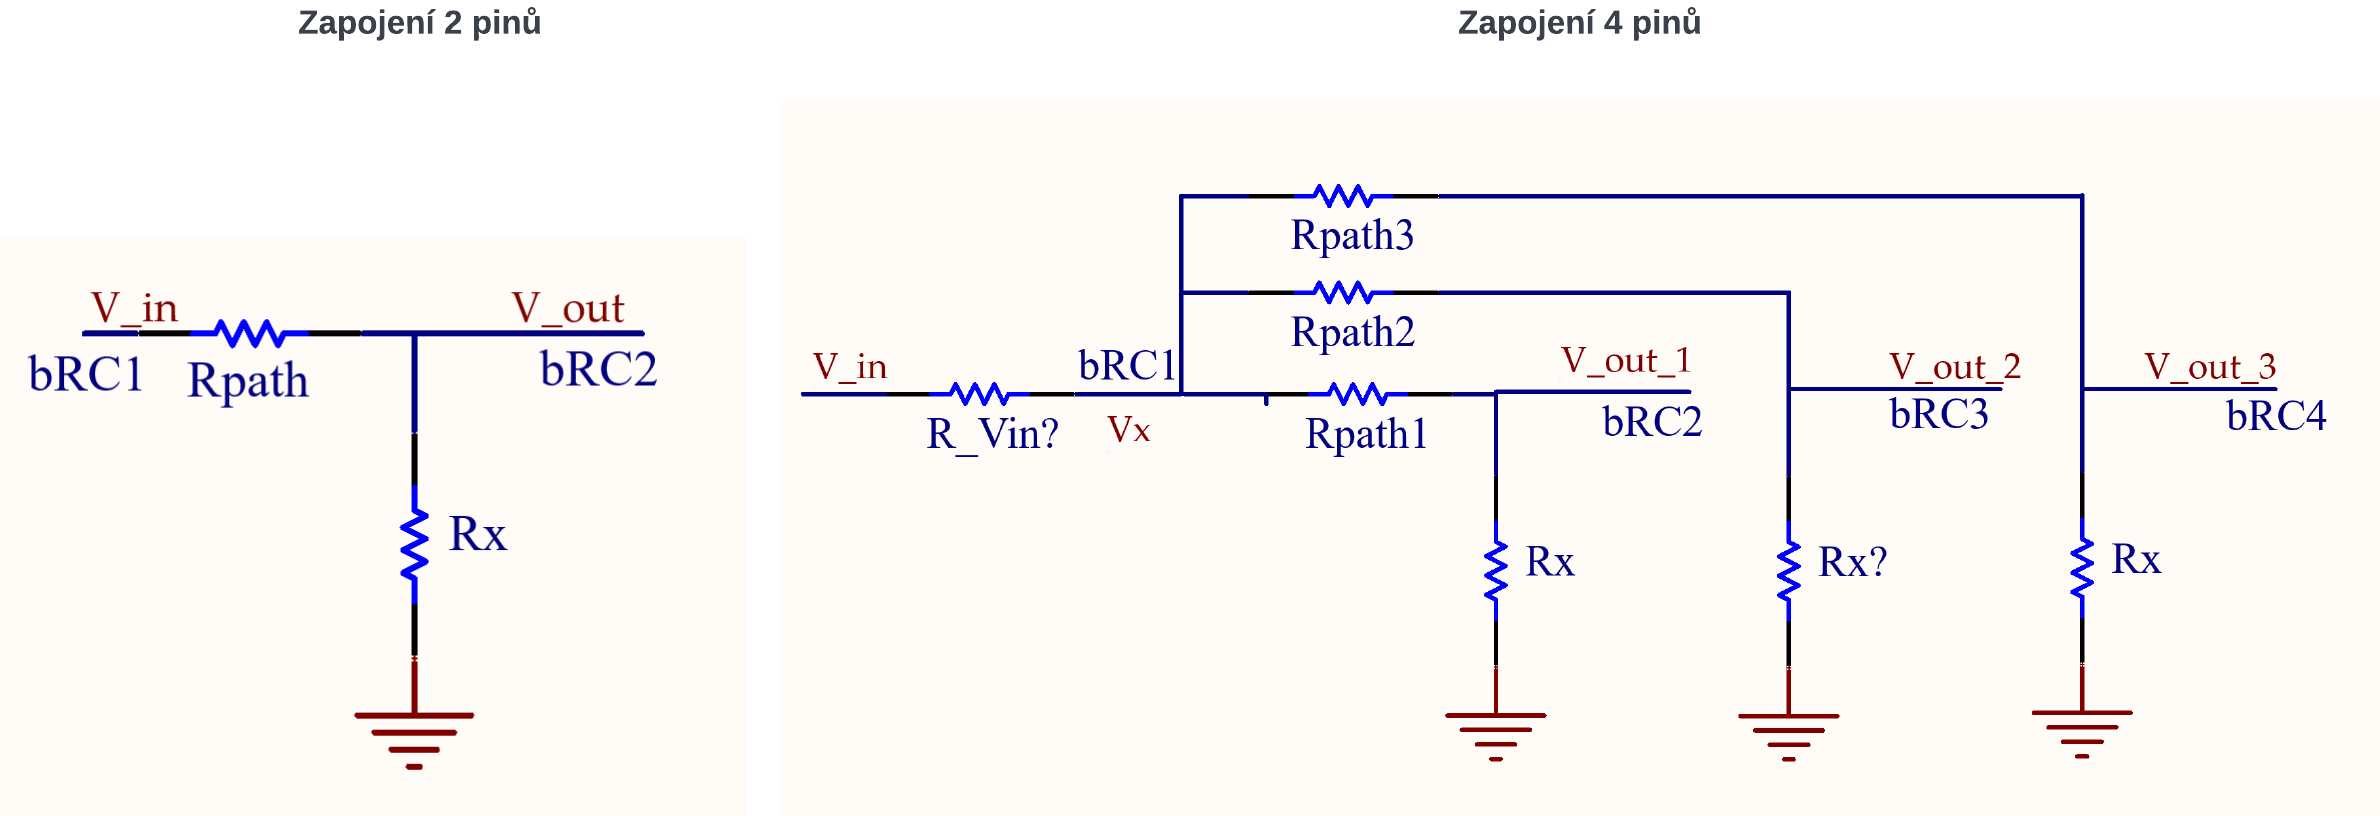
\includegraphics[width = 1\textwidth]{obrazky/2_and_4_pins_connection.png}
            \caption{Napěťový dělič pro 2 a 4 propojené bRC piny}
            \label{fig:Napěťový dělič pro 2 a 4 propojené bRC piny}
    \end{figure}

    Fixture může mít vnitřní zapojení takové, že se vzájemně propojí více než dva bRC piny. V takovém případě by pro např. 4 propojené bRC piny situace
    vypadala jako na obrázku v pravé části, kde odpory Rpath1 až Rpath3 značí odpory jednotlivých cest mezi piny. V\_out\_1 až V\_out\_3 značí napětí na
    výstupech děličů. V případě ideálního zdroje napětí (na obrázku značeno jako Vx) by obvod stále fungoval a platila by
    rovnice \ref{eq:odpor delic} . Do obvodu by však tekl 3-násobný proud.\\
    
    V případě reálného zdroje napětí se uplatňuje jeho vnitřní odpor $R_{Vin}$ a především úbytek napětí vzniklý na tomto odporu.
    Vzhledem k tomu, že úbytek napětí, na vnitřním odporu zdroje, je úměrný protékajícímu proudu a zároveň proud je úměrný počtu propojených pinů, kterých může být
    v případě zemních smyček fixture mnoho. Vzniká potřeba možnosti odpojení jednotlivých bRC pinů. Odpojení bRC pinu je zajištěno pomocí N-channel mosfetu
    \hbox{(obr. \ref{fig:Napěťový dělič pro s možností high Z vstupem}).}
    Toto zapojení v případě nulového napětí na vstupu mosfetu vytvoří vysokou impedanci na vstupu
    pinu, kterým pak protéká pouze zanedbatelný proud. V případě, že je na vstupu napětí vyšší než prahové napětí mosfetu, výpočet odporu se pro ideální zdroj napětí
    změní následovně.
    \begin{equation}
        R_{path} = \frac{(V_{in} - V_{out}) \cdot (R_x + N_{RDSon}) }{V_{out}},
    \end{equation}
     kde $N_{RDSon}$ je odpor otevřeného mosfetu.\\

\clearpage
    \begin{figure}[ht!]
        \centering
        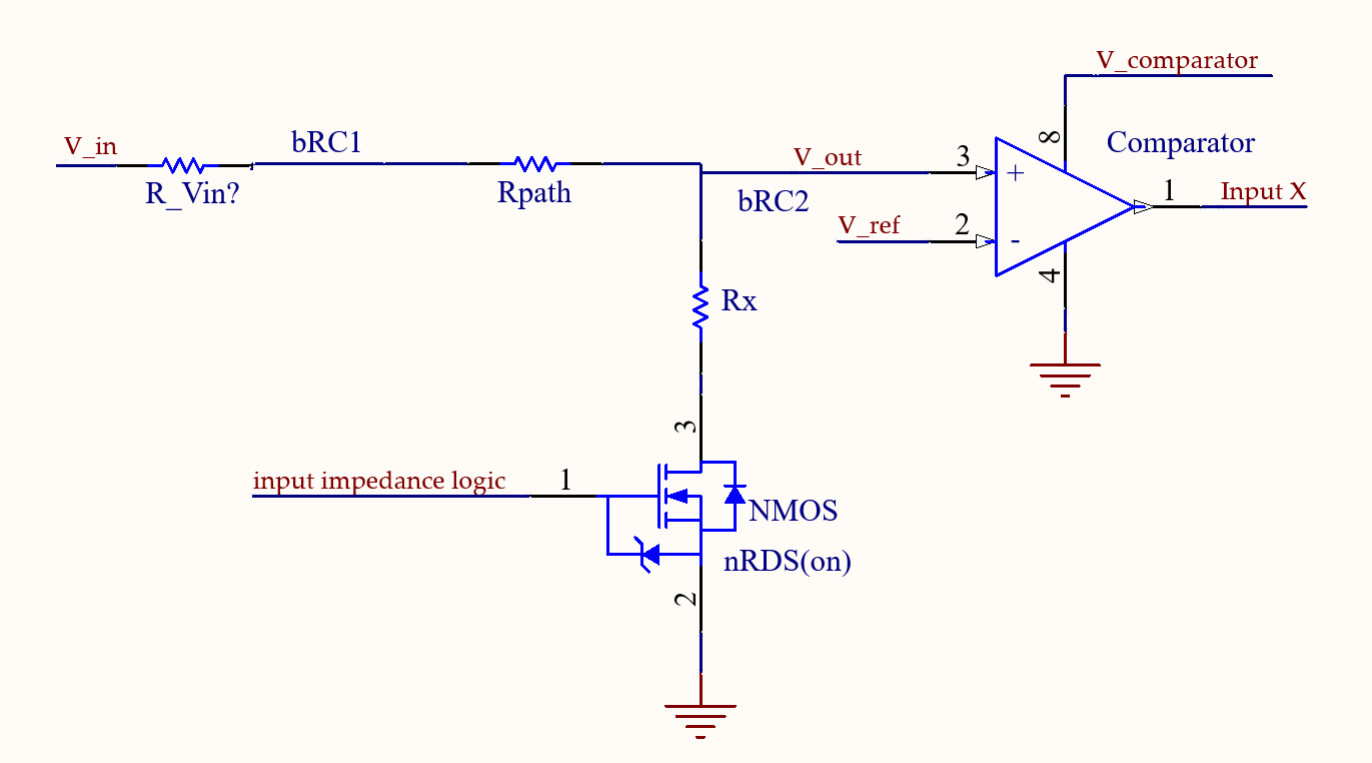
\includegraphics[width = 1\textwidth]{obrazky/nMos_Connection.png}
        \caption{Napěťový dělič pro s možností high Z vstupem}
        \label{fig:Napěťový dělič pro s možností high Z vstupem}
\end{figure}

    Další nevýhodou zapojení na obr.\ref{fig:Napěťový dělič pro 2 a 4 propojené bRC piny}
    je nutnost měření analogového napětí na každém pinu, což by vedlo k
    složitosti zapojení a vysokým nákladům na výrobu. Naprostá většina bRC pinů je propojená jako zkrat a zajímá nás především,
    zda hodnota odporu propojení nepřekračuje nějakou mez.
    Toho lze využít připojením komparátoru na výstup děliče (Obr.\ref{fig:Napěťový dělič pro s možností high Z vstupem}).
    Komparátor porovnává výstupní napětí $V_{out}$ s hodnotou referenčního napětí $V_{ref}$.\\

    Referenční napětí je nastavováno pomocí 12-bit D/A převodníku ovládací desky. V případě nastavení referenčního napětí
    pro určitou mezní hodnotu Rpath,
    lze kontrolovat pouze logickou hodnotu výstupu $V_{comparator}$
    (na obr.\ref{fig:Napěťový dělič pro s možností high Z vstupem} jako InputX).
    V případě, že bude nutné změřit reálný odpor cesty, je možné měnit napětí $V_{ref}$ a sledovat při jaké hodnotě se 
    komparátor překlopí.\\

    Další otázkou je, jak generovat napětí $V_{in}$ na vstupu děliče.
    Protože každý bRC pin musí být zároveň vstupní i výstupní, musí být konfigurovatelný do vysoké impedance (HIGH Z).
    Zároveň pokud bude každý pin schopen dodat do obvodu dostatečné množství proudu,
    bude možné měřit odpor několika cest současně.
    Řešením je obvod na obr.\ref{fig:Zapojení měřící části s p-channel MOSFET}.\\

    V tomto zapojení přibyl P-channel mosfet,
    který umožňuje spínat (ovládat) výstupní napětí V\_in.
    Nicméně vzniká zde obdobný problém jako u zapojení na obr.\ref{fig:Napěťový dělič pro 2 a 4 propojené bRC piny} a to,
    že s rostoucím proudem roste úbytek napětí na vnitřním odporu zdroje charakterizovaným
    odporem $R_{Vin}$. Z tohoto důvodu je úbytek monitorován 12 bitovým A/D převodníkem (na ovládací kartě).
    Výsledek měření odporu je pak vztažen k hodnotě změřené pomocí A/D převodníku.
    Odpor zdroje se pak bude rovnat $R_{DSon}$ P-channel mosfetu.
    Nastává tak problém určit vliv odporu $R_{DSon}$ na výslednou hodnotu změřeného odporu Rpath\cite{HOROWITZ,MARTINT}.
    \clearpage

    Protože každý pin může být zároveň výstupní i vstupní, kde vstupní funkci plní lokální komparátor.
    Lze pro přesné měření změřit přímo výstupní napětí V\_out\_local pomocí lokálního komparátoru a vliv $R_{DSon}$ úplně eliminovat.
    Nicméně tato metoda je časově náročnější a je více diskutována v kapitole o algoritmizaci.\\
        
    %\noindent
    %$R_{path} = \frac{V_{ADC} \cdot (R_{NMOS}+ R_{X}) }{V_{out}} - R_{NMOS} - R_{X} - R_{PMOS}$,\\\\
    %kde $R_{NMOS}$ a $R_{PMOS}$ jsou hodnoty RDSon otevřených P a N mosfetů.\\
\begin{figure}[ht!]
        \centering
        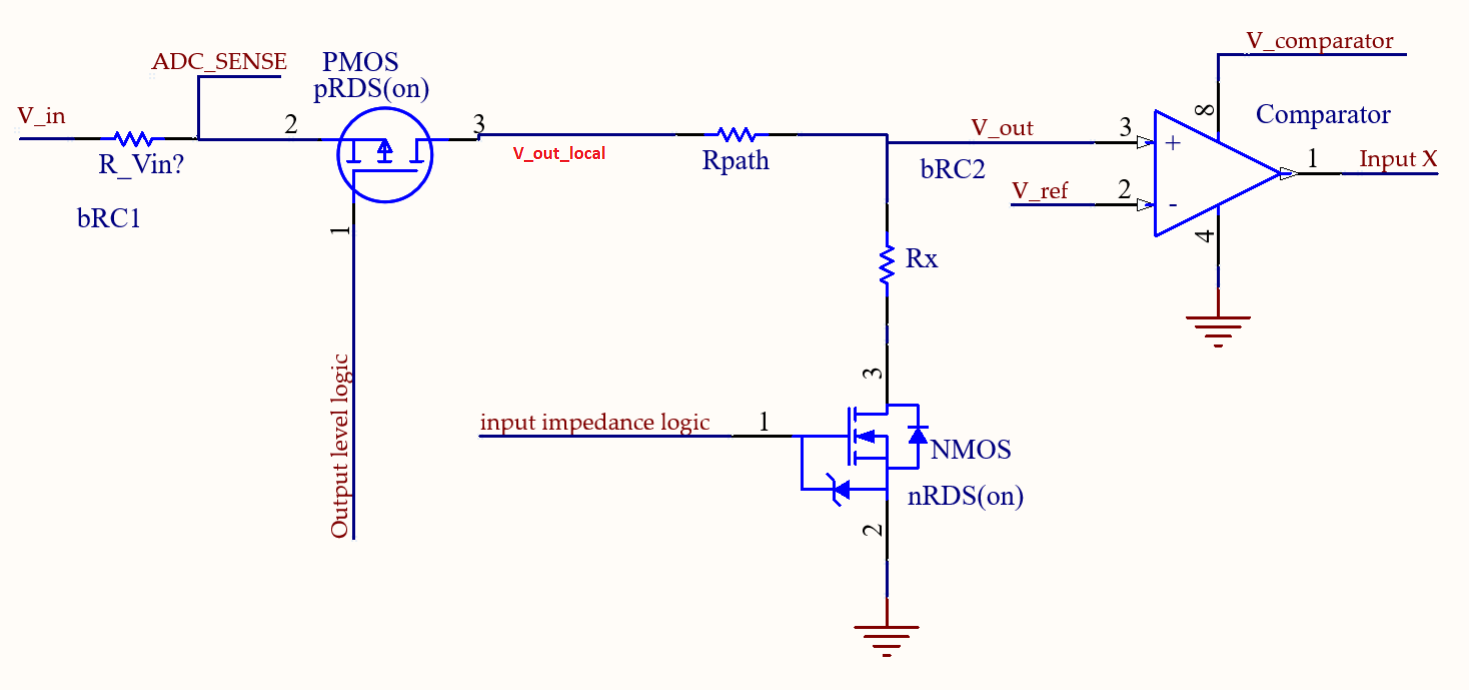
\includegraphics[width = 1\textwidth]{obrazky/final_connection.png}
        \caption{Zapojení měřící části s p-channel MOSFET}
        \label{fig:Zapojení měřící části s p-channel MOSFET}
\end{figure}

    Ve schématu na obr.\ref{fig:Zapojení měřící části s p-channel MOSFET}
    si lze všimnout řídících napětí (Output level logic, input impedance logic a input X).
    Output level logic řídí, zda generuje rBC pin napětí.
    Input impedance logic umožňuje nastavit HIGH Z na vstupním obvodu. Input X je výstup komparátoru. Vzniká
    tak potřeba pro každý bRC pin mít 2 logické výstupy a jeden vstup. Každá deska musí mít minimálně 78 bRC pinů,
    což znamená minimálně 156 logických výstupů a 78 logických vstupů.\\

    Pro tento účel je použito pro nastavení 78x Output level logic 2x5x8-bit shift registrů zapojených do série.
    Obdobně je pro nastavení 78x input impedance logic je použito 2x5x8-bit shift registrů zapojených do série.
    a pro 78 logických výstupů je použito 2x5x8-bit multiplexerů se společnou adresací.
    Společnou adresací se rozumí, že adresy 2x5 multiplexerů jsou řízeny 2x3 adresními piny.
    Vzhledem k použití 8-bit komponentů je výsledný počet bRC pinů na desce zaokrouhlen na 80 místo 78,
    přičemž 2 poslední vstupy/výstupy jsou na testeru ignorovány
    (v případě měřící desky č.1 je pin č. 80 použit pro externí sondu). 
    Hierarchické schéma měřící karty lze nalézt v příloze.\\

    Měřící karty fungují, vzhledem k potřebám testování, ve dvou režimech (PASS/FAIL a měření reálného odporu).
    PASS/FAIL režim je určen pro rychlé hromadné otestování všech pinů,
    kde hlavním kritériem je, zda propojení mezi piny odpovídají nějaké mezní hodnotě odporu nebo ne.
    Výsledkem je pak pouze mapa propojení bez hodnot reálného odporu.
    Režim měření reálného odporu pak umožňuje změřit co nejpřesnější hodnotu odporu všech propojení.
\clearpage
\subsubsection{Výběr součástek a volba jejich hodnoty}
V předchozí sekci byla diskutována funkčnost zapojení.
Nicméně nebylo doposud zmíněno, jaké kvantitativní hodnoty součástek jsou vhodné pro realizaci.
V této sekci jsou popsány konkrétní reálné součástky, které byly použity včetně zdůvodnění jejich výběru.\\

\subsubsection{Volba velikosti odporu děliče Rout}
\textbf{Odvození podmínek pro výběr odporu děliče:}\\
V celé následující sekci je zanedbán vliv komparátoru na měřící obvod.
V první řadě je nutné definovat jaká je vyžadovaná přesnost, rozsah a rychlost měření.
Vzhledem k charakteru propojení ve fixture by měl být tester schopen změřit odpor v rozsahu od 1\,$\Omega$ do 1\,k$\Omega$.
Vyžadované rozlišení je 1$\Omega$ především pro odpory do 100\,$\Omega$.
Co se týče rychlosti měření, tak pro automatické měření mezi dvěma bRC piny nejsou kladeny žádné požadavky,
protože je proces plně automatizován.\\
Při měření odporu mezi bRC a Probe piny, obsluha postupně testuje všechny piny všech karet zvlášť externí sondou.
V tomto případě by prodleva mezi přiložením sondy a vyhodnocením signálu neměla být pro
člověka rozpoznatelná (signalizace pískáním obdobně jako continuity test multimetru).
Z tohoto důvodu je nutné pro jeden pin změřit propojení mezi všemi ostatními piny
do cca 40\,ms (včetně komunikací s PC cca. 30\,ms).
Nicméně stačí vyhodnocovat PASS/FAIL pro odpor cesty a ne přímo jeho hodnotu.
Následující tabulka je shrnutím tohoto odstavce.\\


\begin{table}[ht!]
    \resizebox{\textwidth}{!}{%
    \begin{tabular}{|lccccc|}
    \hline
    \multicolumn{6}{|c|}{\textbf{Požadované charekteristiky měřícího obvodu}}                                                                                                                                                                                                                                                                                  \\ \hline
    \multicolumn{1}{|l|}{\textbf{TEST MODE}}                & \multicolumn{1}{c|}{\textbf{Počet pinů}} & \multicolumn{1}{c|}{\textbf{Rozsah $[\Omega]$}}  & \multicolumn{1}{c|}{\textbf{Přesnost $[\pm \Omega]$}} & \multicolumn{1}{c|}{\textbf{čas $[\mu s/pin]$}} & \textbf{Celkový čas $[ms]$} \\ \hline
    \multicolumn{1}{|l|}{\textbf{PASS/FAIL}}                & \multicolumn{1}{c|}{4000}                & \multicolumn{1}{c|}{1-1000}                      & \multicolumn{1}{c|}{2}                                & \multicolumn{1}{c|}{2,5}                        & 10                          \\ \hline
    \multicolumn{1}{|l|}{\textbf{Měření   "pravé"\ hodnoty}} & \multicolumn{1}{c|}{4000}                & \multicolumn{1}{c|}{1-1000}                      & \multicolumn{1}{c|}{1}                                & \multicolumn{1}{c|}{Nedefinován}                & Nedefinován                 \\ \hline
    \end{tabular}%
    }
    \caption{Požadované měřící charakteristiky}
    \label{tab:Požadované měřící charakteristiky}
\end{table}

Všechna následující odvození vycházejí z následující výchozí rovnice pro výstup napěťového děliče pro 2 propojené bRC piny:

\begin{equation}
V_{out} = \frac{ V_{in}\cdot R_{out} }  {R_{out} + R_{path} + R^P_{DSon}},
\end{equation}

kde ${R_{out}} = R_X + R^N_{DSon}$ a $R^P_{DSon}$ je ekvivalent $R_{Vin}$ a odpovídá odporu P-channel mosfetu. \\

Z tabulky vyplývá několik podmínek pro volbu rezistoru ${R_{out}}$. První podmínka se vztahuje k přesnosti měření. Přesnost měření ovlivňují převážně 2 faktory.
Prvním faktorem je chyba vzniklá diskretizací referenčního napětí komparátoru,
které je generováno 12bit D/A převodníkem. Protože rovnice pro výstupní napětí děliče je nelineární
bude nelineární i chyba vzniklá kvantováním. Podmínku pro splnění přesnosti, v případě, že se projeví pouze kvantizační chyba, lze vyjádřit následovně:

\begin{equation}
\left| \frac{\partial V_{out} }{\partial R_{path}}\cdot \Delta R_{path} \right| > \frac{V_{ref}}{2^{12}},
\end{equation}

kde $\left| \frac{\partial V_{out} }{\partial R_{path}}\cdot \Delta R_{path} \right|$
značí změnu napětí Vout způsobenou změnou $R_{path}$ o
požadovanou přesnost v $\Omega$ a $R_{path}$ je z rozsahu 0 - 1k\,$\Omega$.
Tento vztah se také dá reprezentovat jako citlivost měření na změnu $R_{path}$.\\

Druhým faktorem, ovlivňujícím přesnost je chyba, kterou do měření přidává odpor $R^P_{DSon}$ P-channel mosfetu při paralelním měření několika bRC pinů.
Tato chyba roste s zvyšujícím se proudem a projeví se tak především při PASS/FAIL režimu.
Vzhledem k náhodnému vnitřnímu propojení fixture není možno dopředu odhadnout, kolik bRC pinů bude připojeno a tak ani výsledný proud odporem $R^P_{DSon}$.
Uvažujme, že chceme změřit "nejhorší scénář"\ (všechny piny jsou mezi sebou propojeny tvrdým zkratem).
Následně poteče obvodem proud přibližně:

\begin{equation}
I = \frac{V_{in}}{R_{out}/N_{pins} + R^P_{DSon}}
\end{equation}

 Proud je tak nepřímo úměrný velikosti hledaného odporu Rout a počtu paralelně měřených pinů.
 Pokud bychom chtěli změřit všechny piny na kartě současně ($N_{pins}$ = 80).
 Musí každý pin být schopen dodat do obvodu proud $I = 80 \cdot V_{in}/R_{out}$.
 Vzhledem k nenulovému odporu $R^P_{DSon}$, který lze připodobnit
 vnitřnímu odporu zdroje napětí vzniká následující podmínka pro nejhorší možný případ:

 \begin{equation}
    I \cdot {R^P_{DSon}}  < \left| \frac{\partial V_{out} }{\partial R_{path}}\cdot \Delta R_{path} \right|\
\end{equation}

\begin{equation}
   \frac{V_{in} \cdot R^P_{DSon}}{R_{out}/N_{pins} + R^P_{DSon}} < \left| \frac{\partial V_{out} }{\partial R_{path}}\cdot \Delta R_{path} \right|
\end{equation}
Podmínka vyjadřuje, že chyba vzniklá úbytkem napětí na $R^P_{DSon}$ za předpokladu Npins propojených pinů,
by na výstupu děliče Vout neměla být větší než nejnižší napětí, které vznikne změnou odporu cesty o požadovanou přesnost v\,$\Omega$. \\

Při uvážení nejhoršího scénáře, že se sečte chyba dána kvantováním a chyba dána odporu $R^P_{DSon}$, lze vyjádřit podmínku pro hledaný odpor
$R_{out}$ následovně:

\begin{equation}\label{eq:citilivost}
\frac{V_{ref}}{2^{12}} + \frac{V_{in} \cdot R^P_{DSon}}{R_{out}/N_{pins} + R^P_{DSon}} < \left| \frac{\partial V_{out} }{\partial R_{path}}\cdot \Delta R_{path} \right|
\end{equation}
\\
\textbf{Řešení podmínek výběru hodnoty odporu děliče:}\\
    Rovnici \ref{eq:citilivost} lze považovat za citlivost obvodu na změnu odporu $R^P_{DSon}$.
    Řešením by měla být být oblast hodnot, ve které odpor $R_{out}$ splňuje podmínky pro přesnost.
    Kvůli názornosti byla zvolena grafická metoda řešení.
    Následující obrázek \ref{fig:3D zobrazení rovnice pro výstupní napětí děliče}
    ukazuje výstupní napětí ideálního děliče v závislosti na odporu $R_{out}$ a $R_{path}$.
    V levé části je zobrazena celá zkoumaná oblast a v pravé části je stejný graf zobrazen z "bočního"\ pohledu.
    V takovém zobrazení je patrné, jaká je změna výstupního napětí $V_{out}$ při změně odporu $R_{path}$.
    Pokud zobrazíme 2 sousední hodnoty výstupního napětí tak, aby náležely stejnému odporu $R_{out}$ (leží vertikálně nad sebou).
    Rozdílem těchto 2 hodnot získáme citlivost
    $\left| \frac{\partial V_{out} }{\partial R_{path}}\cdot \Delta R_{path} \right|$.
    Na obrázku je z důvodu lepšího zobrazení zvolena velká změna odporu $\Delta R_{path}$
    (v tomto případě 20\,$\Omega$).
    Pro správný návrh je pak nutné zvolit stejnou změnu odporu $\Delta R_{path}$ jako má požadovaná přesnost\cite{Sensitivity_embedded,Sensitivity_2}.\\

\begin{figure}[ht!]
    \centering
    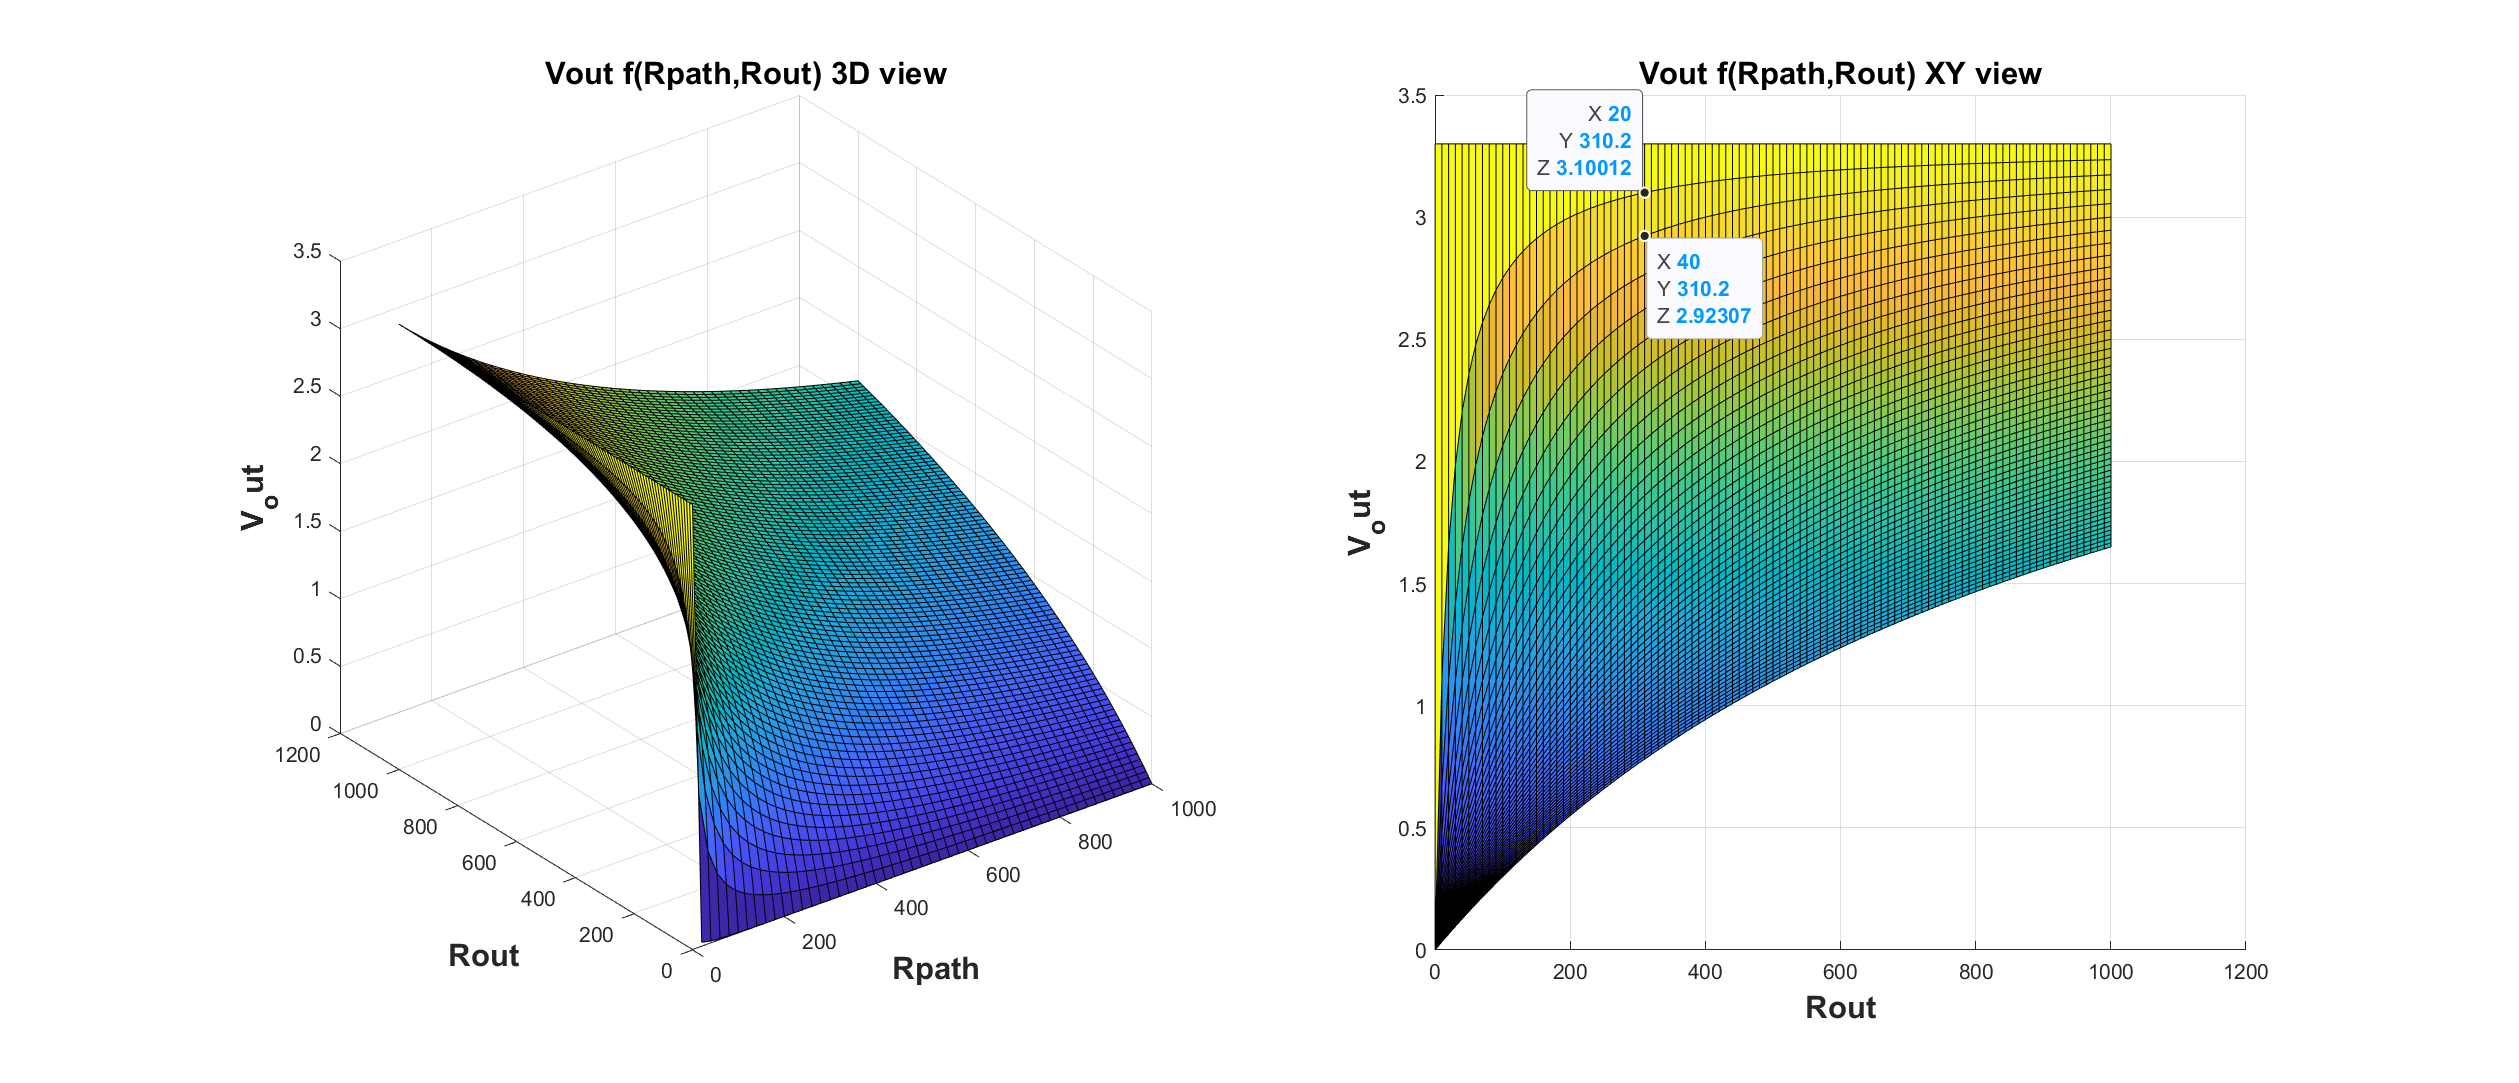
\includegraphics[width = 1\textwidth]{obrazky/Vout3D.eps}
    \caption{3D zobrazení rovnice pro výstupní napětí děliče (generováno pomocí MATLAB) }
    \label{fig:3D zobrazení rovnice pro výstupní napětí děliče}
\end{figure}

Nyní přejděme k řešení rovnice (\ref{eq:citilivost}). Následující obrázek \ref{fig: zobrazení df/dRpath}
zobrazuje ve své levé části zeleně hodnotu citlivostí $\frac{ \Delta V_{out} }{\Delta R_{path}}$
v celém zkoumaném prostoru. Červeně je pak zobrazena druhá strana rovnice (\ref{eq:citilivost}).
Podmínky jsou splněny ve všech kombinacích odporu $R_{out}$ a $R_{path}$, kde má zelená část
vyšší hodnoty diference než červená.
V pravé části obrázku je pro jednodušší odečítání hodnot odporu výsledné oblasti pohled "shora".
Zelená oblast splňuje podmínky a červená nesplňuje.
Obecně platí, čím hlouběji v zelené oblasti se zkoumaný bod nachází, tím vyšší je přesnost\\

\begin{figure}[ht!]
    \centering
    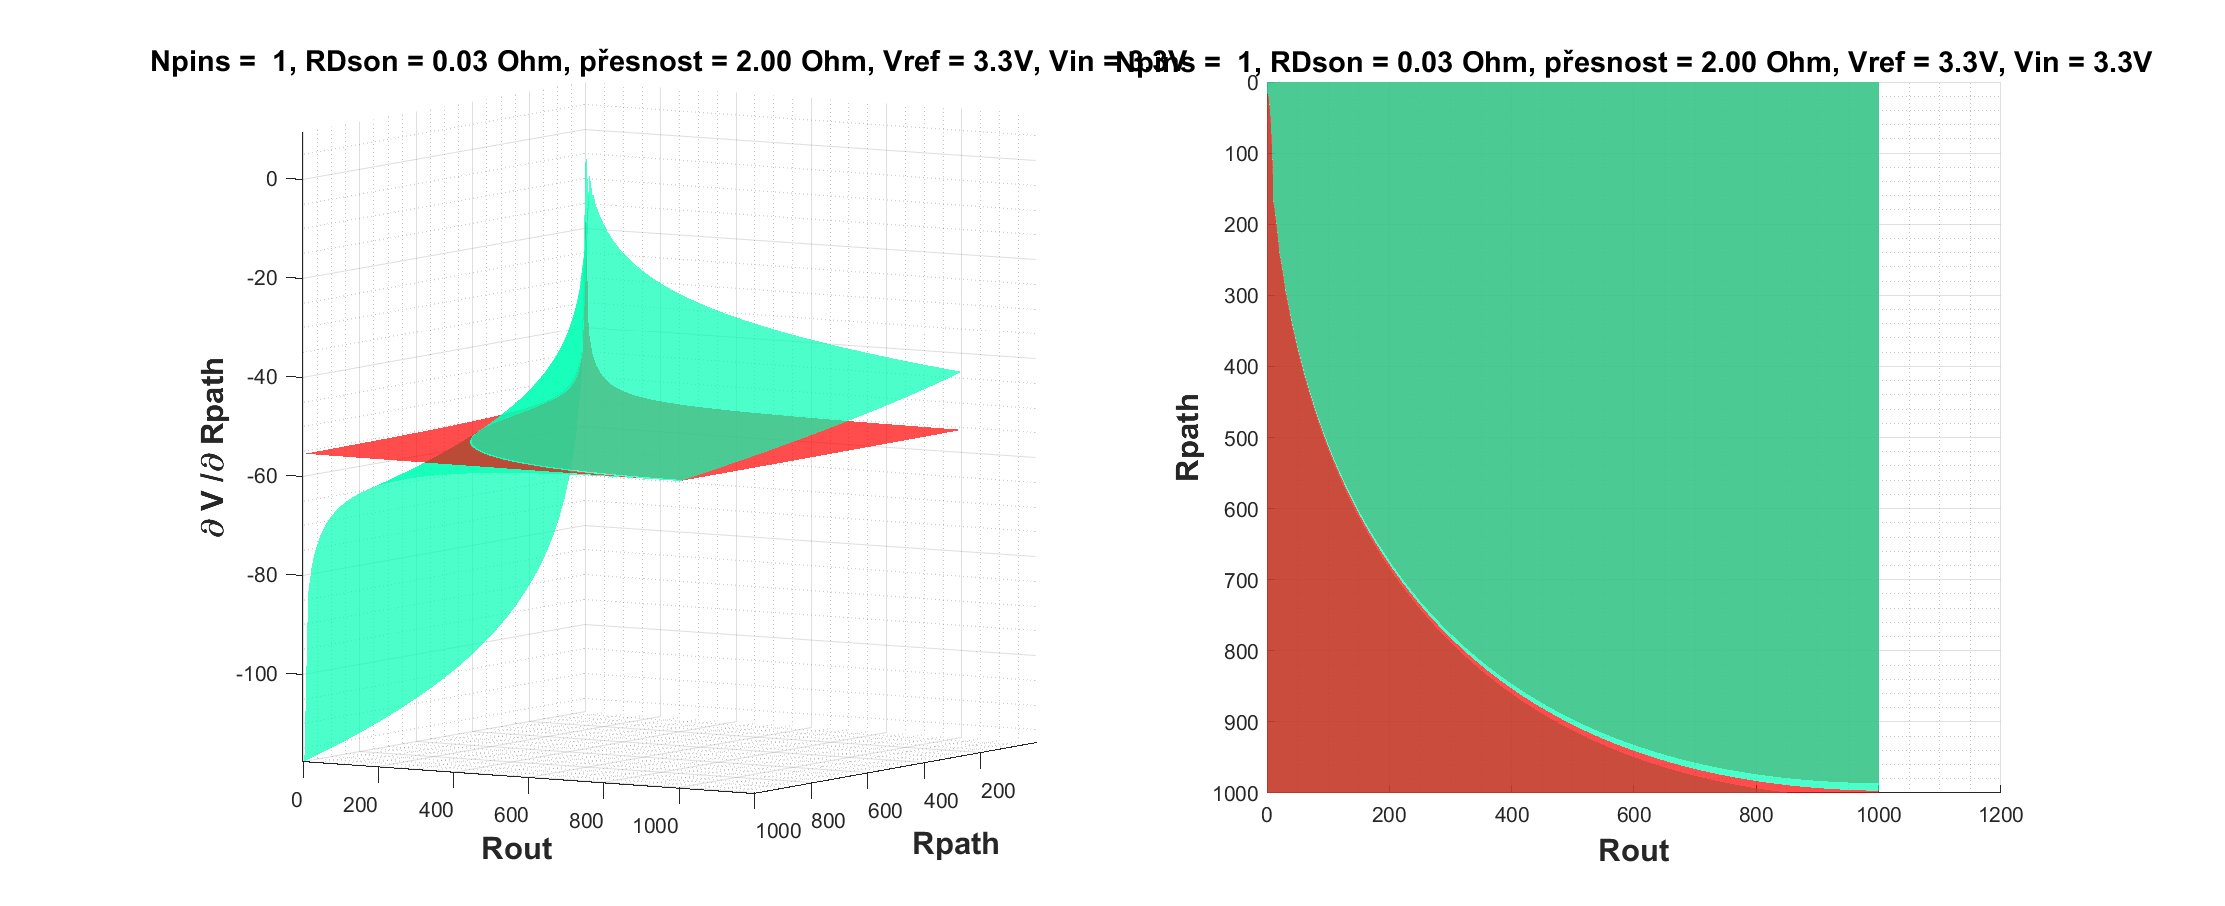
\includegraphics[width = 1\textwidth]{obrazky/general_dVF.eps}
    \caption{3D zobrazení rovnice \ref{eq:citilivost} s podmínkami (generováno pomocí MATLAB)}
    \label{fig: zobrazení df/dRpath}
\end{figure}

Do rovnice však vstupují parametry, jako je počet paralelně měřených pinů,
odpor $R^P_{DSon}$ a volba přesnosti. Následující série grafů zobrazuje vliv
těchto parametrů na výslednou oblast, která splňuje podmínky.
Výsledný zvolený odpor je 400$\Omega$ a v grafech jsou krajní hodnoty pro tento bod označeny
(x: $R_{path}$, y: $R_{out}$ a  z: $20log(\left| \frac{\partial V_{out} }{\partial R_{path}}\cdot \Delta R_{path} \right|$) ).\\
\clearpage

Zkoumání vlivu počtu pinů nás zajímá především při provozu testeru v PASS/FAIL režimu,
kdy je nutné provádět měření rychle. Zároveň zde máme definovanou maximální chybu měření
do 2$\Omega$. Při tomto testu se předpokládá, že všechny měřené cesty mají odpor do 100 $\Omega$.
Z obrázku \ref{fig:PASS_FAIL 2 OHMS MEASUREMENT} je patrné, že nebude možné
změřit všech 80 pinů jedné karty současně s požadovanou přesností.
Požadovanou přesnost nebude možné dosáhnout ani při měření 60 pinů současně, protože nejvyšší hodnota odporu cesty,
která leží v zelené oblasti je přibližně 60\, $\Omega$.
Při této úvaze bylo počítáno s $R^P_{DSon} = 0.03\Omega$, což je hodnota o cca 15m$\Omega$ vyšší než má použitý P - channel mosfet.
(Výběr mosfetu je dále v diplomové práci).
Hodnota zvoleného odporu 400$\Omega$ umožňuje,při měření 40 pinů současně, splnit podmínku přesnosti $\pm 2\Omega$ pro určení hodnoty odporu propojení do přibližně 220
$\Omega$.\\



\begin{figure}[ht!]
    \centering
    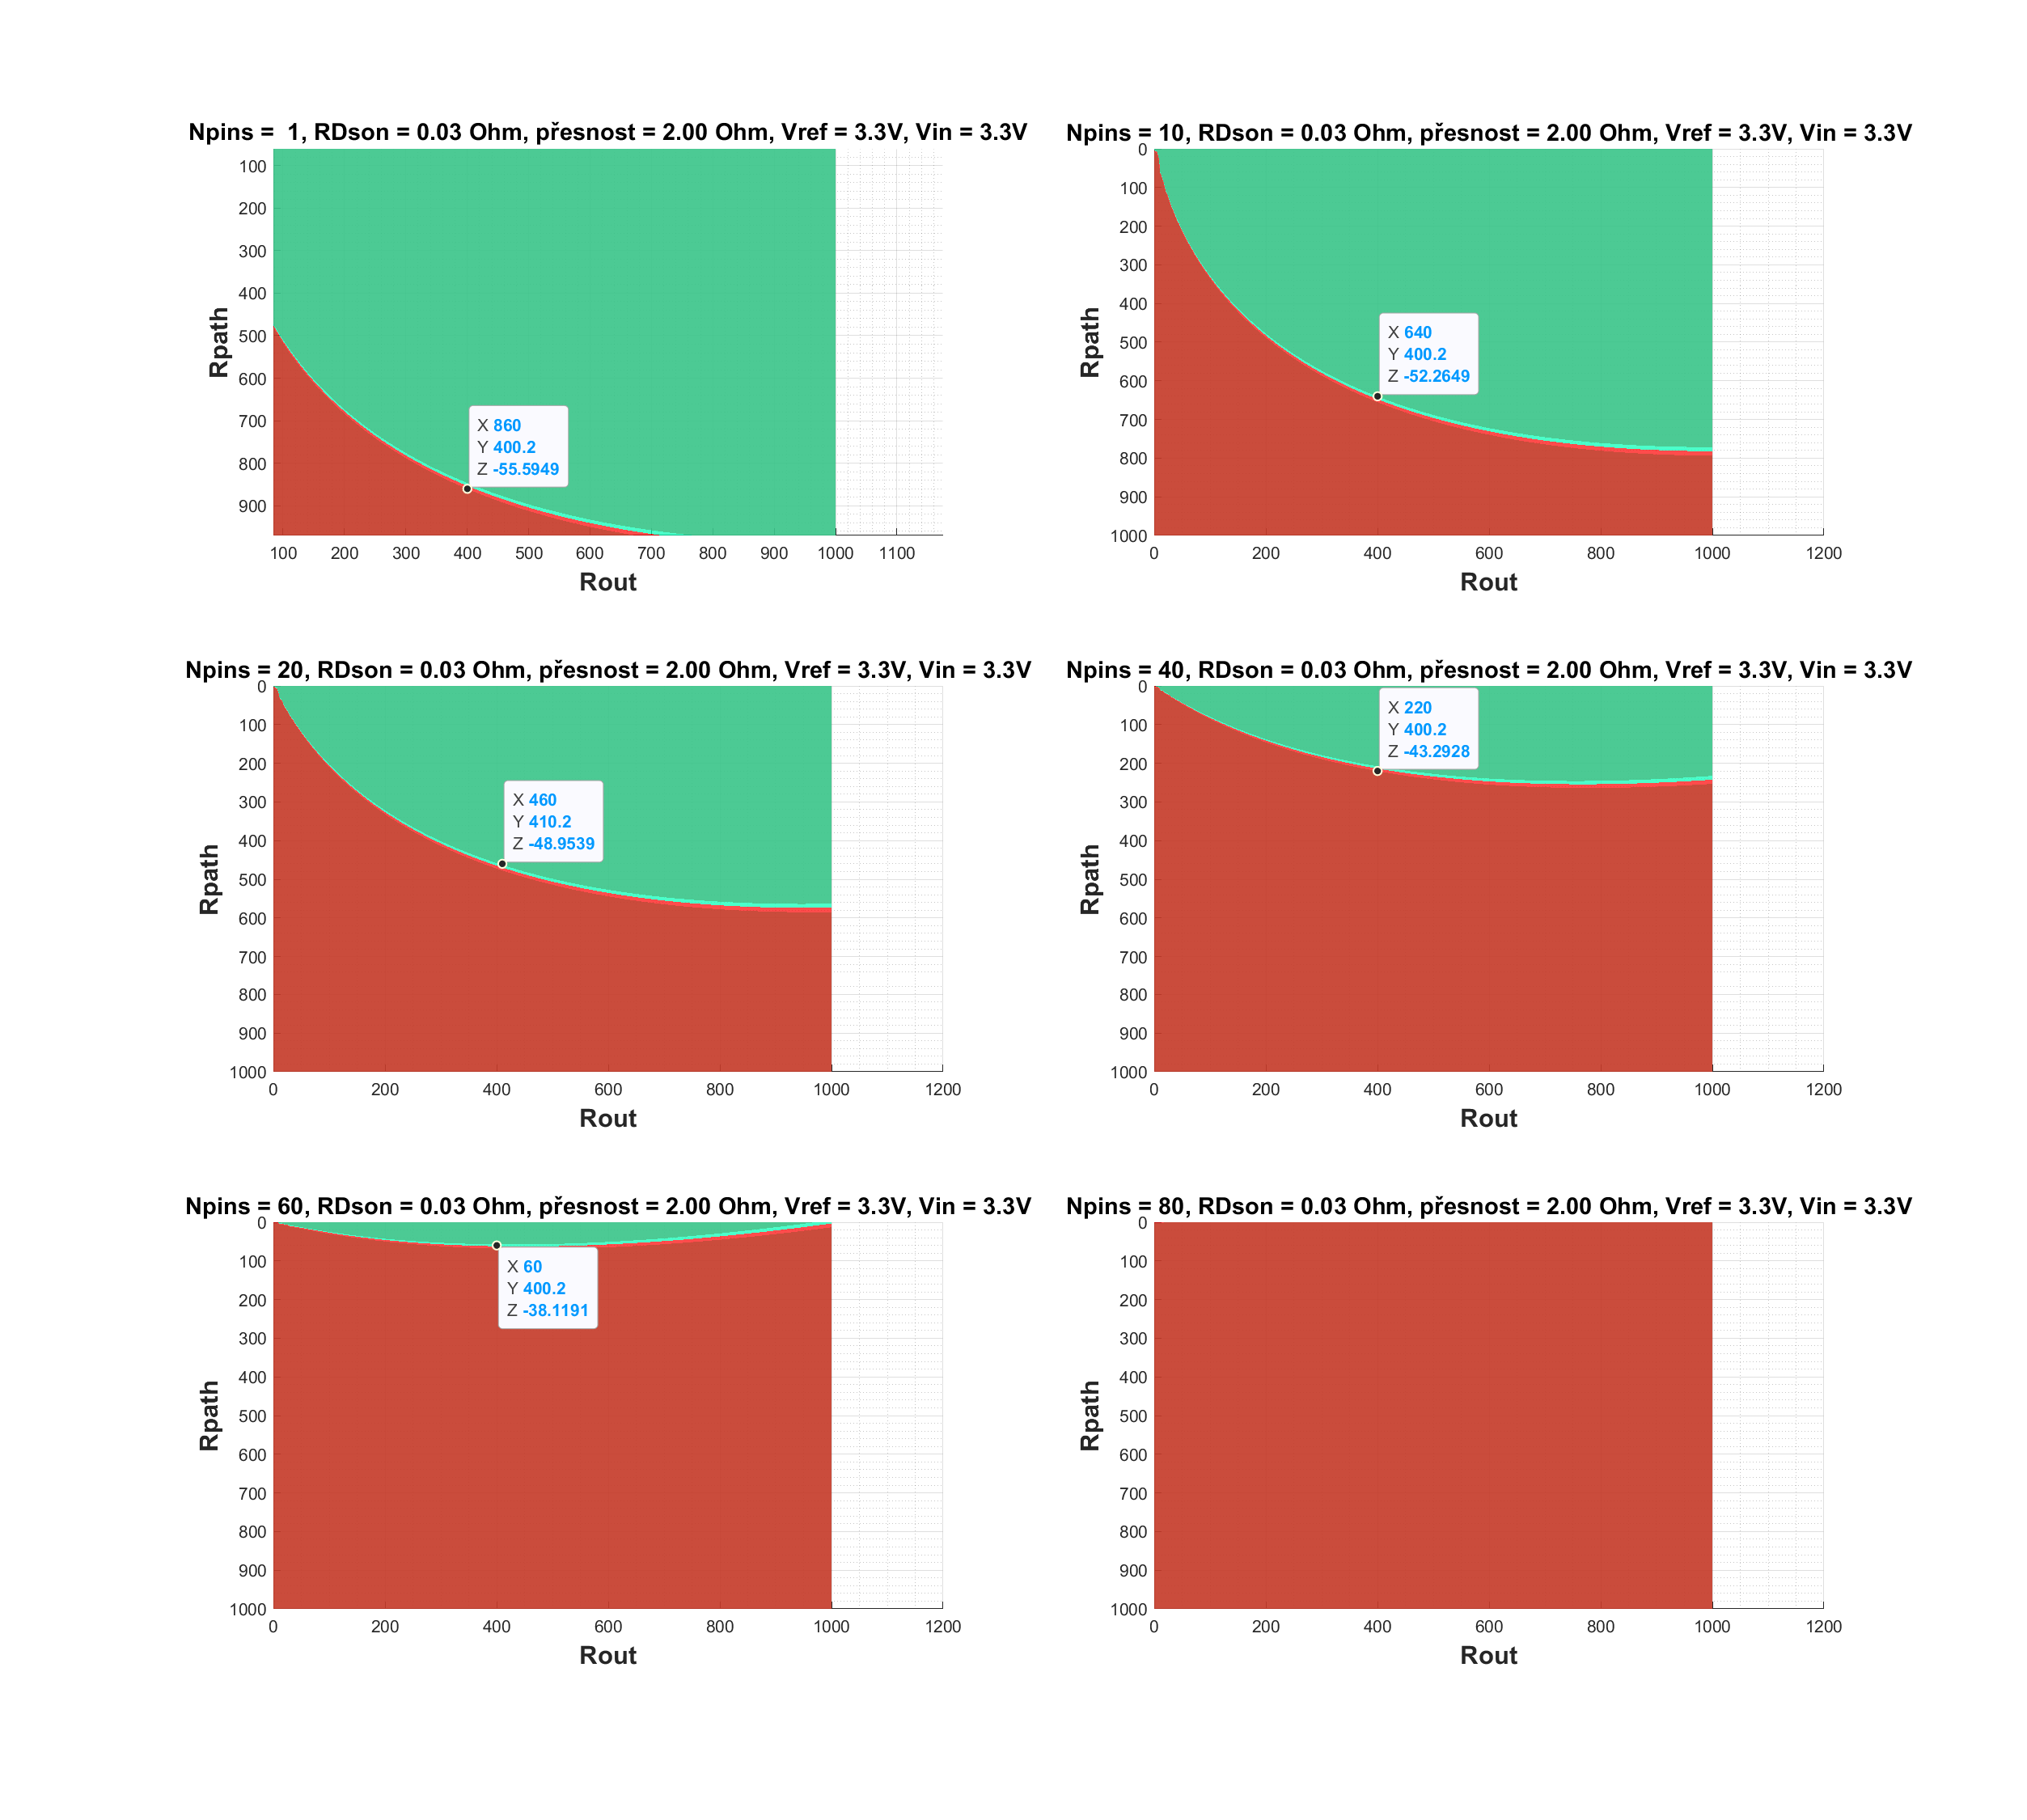
\includegraphics[width = 1\textwidth]{obrazky/PASS_FAIL_MERENI.eps}
    \caption{PASS FAIL -  přesnost $R_{path}$ 2$\Omega$ (generováno pomocí MATLAB)}
    \label{fig:PASS_FAIL 2 OHMS MEASUREMENT}
\end{figure}

\clearpage
Vliv požadované přesnosti měření nás zajímá v režimu vyhodnocení co nejpřesnější hodnoty měřené cesty.
V tomto režimu se předpokládá měření propojení pouze 2 pinů.
Z obrázku \ref{fig:One pin MEASUREMENT} je patrné, že vyšší přesnosti lze docílit volbou nižšího odporu $R_{out}$.
Tento požadavek je protichůdný s požadavkem na velikost odporu pro PASS/FAIL test(\ref{fig:PASS_FAIL 2 OHMS MEASUREMENT}).
Hodnota výsledného odporu 400$\Omega$ tak byla zvolena jako jistý kompromis mezi těmito dvěma požadavky.

\begin{figure}[ht!]
    \centering
    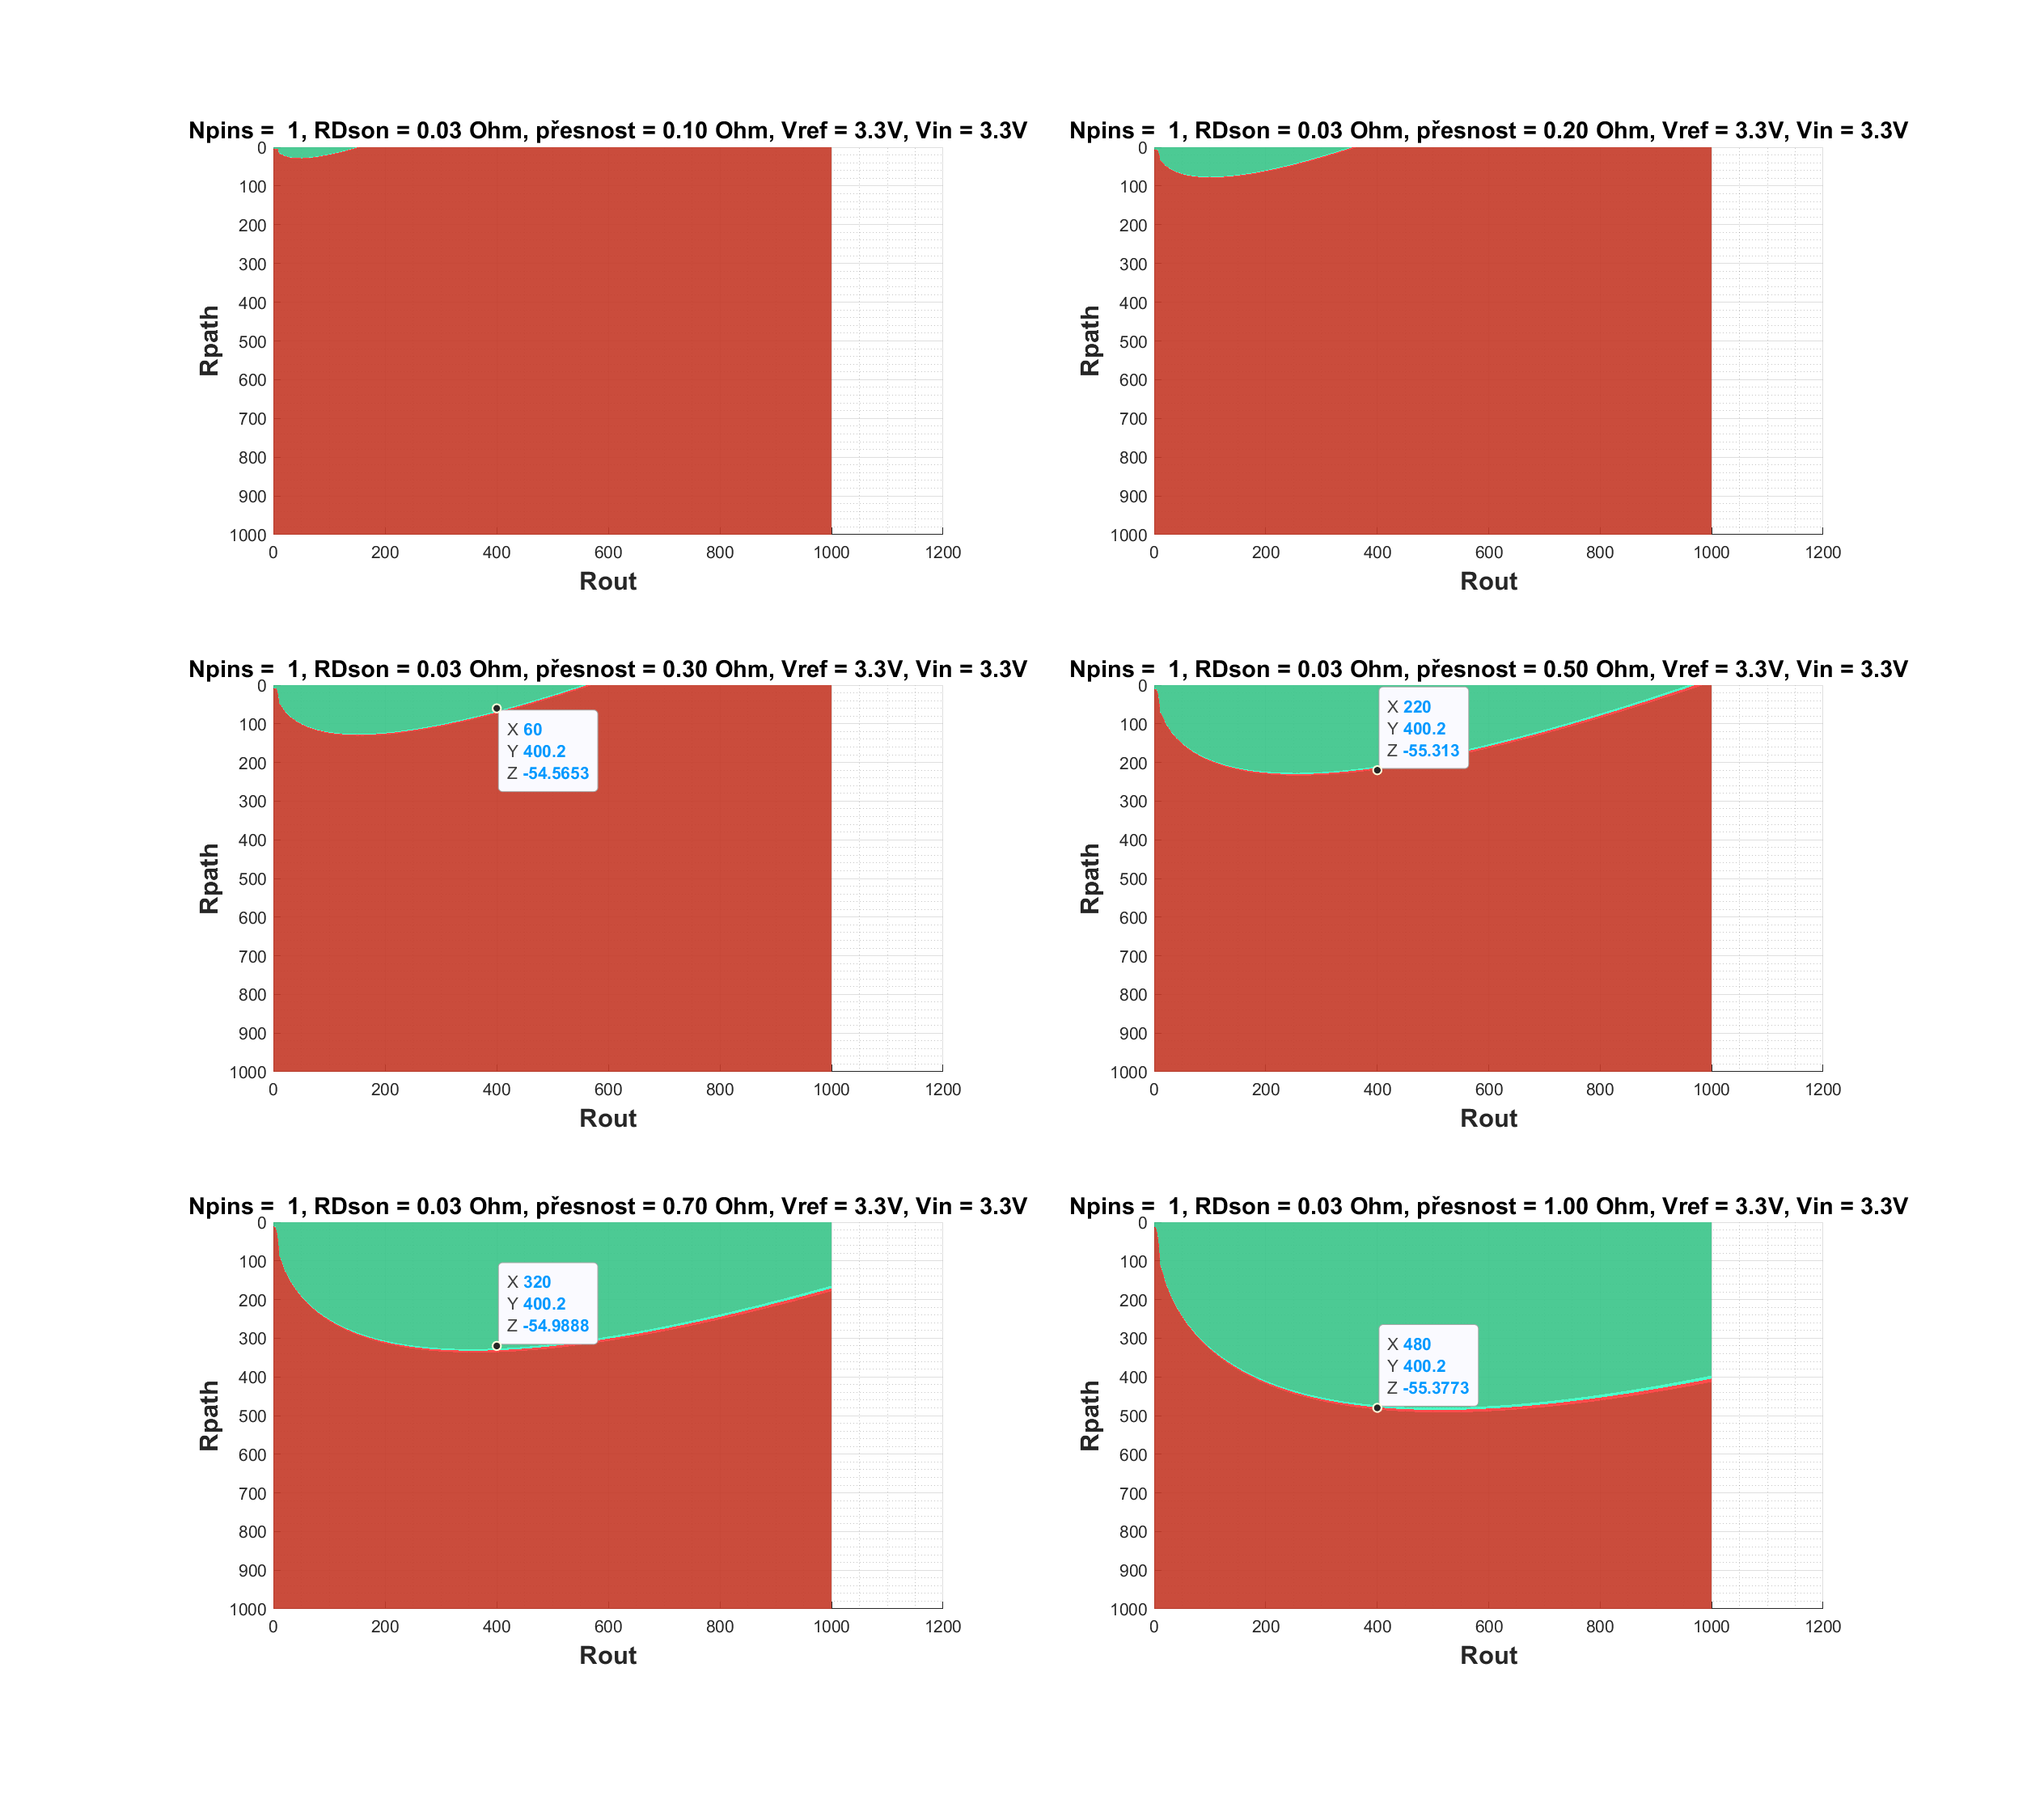
\includegraphics[width = 1\textwidth]{obrazky/MERENI_JEDNOHO_PINU.eps}
    \caption{Přesné měření mezi 2 piny - (generováno pomocí MATLAB)}
    \label{fig:One pin MEASUREMENT}
\end{figure}
\clearpage



\subsubsection{Volba P-channel mosfetu}
Při výběru P-channel mosfetu je vzhledem k podmínkám na přesnost nutné zvolit mosfet s nízkým odporem $R^P_{DSon}$.
Tohoto odporu by mělo být možno dosáhnout pomocí řídícího napětí 3.3V.
Zároveň by měl mosfet být schopen dodat do obvodu dostatečný proud pro měření 40 pinů současně (proč 40 pinů je zdůvodněno v kapitole
o volbě odporu $R_{out}$). Mosfet musí tedy do obvodu být schopen dodat následující minimální proud.

\begin{equation} \label{eq:MIN_CURRENT}
    I_{min} = \frac{40 \cdot V_{in}}{R_{out}} = \frac{40 \cdot 3.3}{400} = 330mA
\end{equation}

 Z následujícího obrázku je patrné, že při použití $R_{out} = 400\Omega$ je pro splnění podmínky přesnosti měření 2$\Omega$ v rozsahu od 1 do 100$\Omega$ zvolit mosfet s
 nejvyšším možným $R^P_{DSon}$ přibližně 0.032$\Omega$. Zároveň je zde požadavek na co nejnižší cenu, dostupnost a menší velikost pouzdra. 

\begin{figure}[ht!]
    \centering
    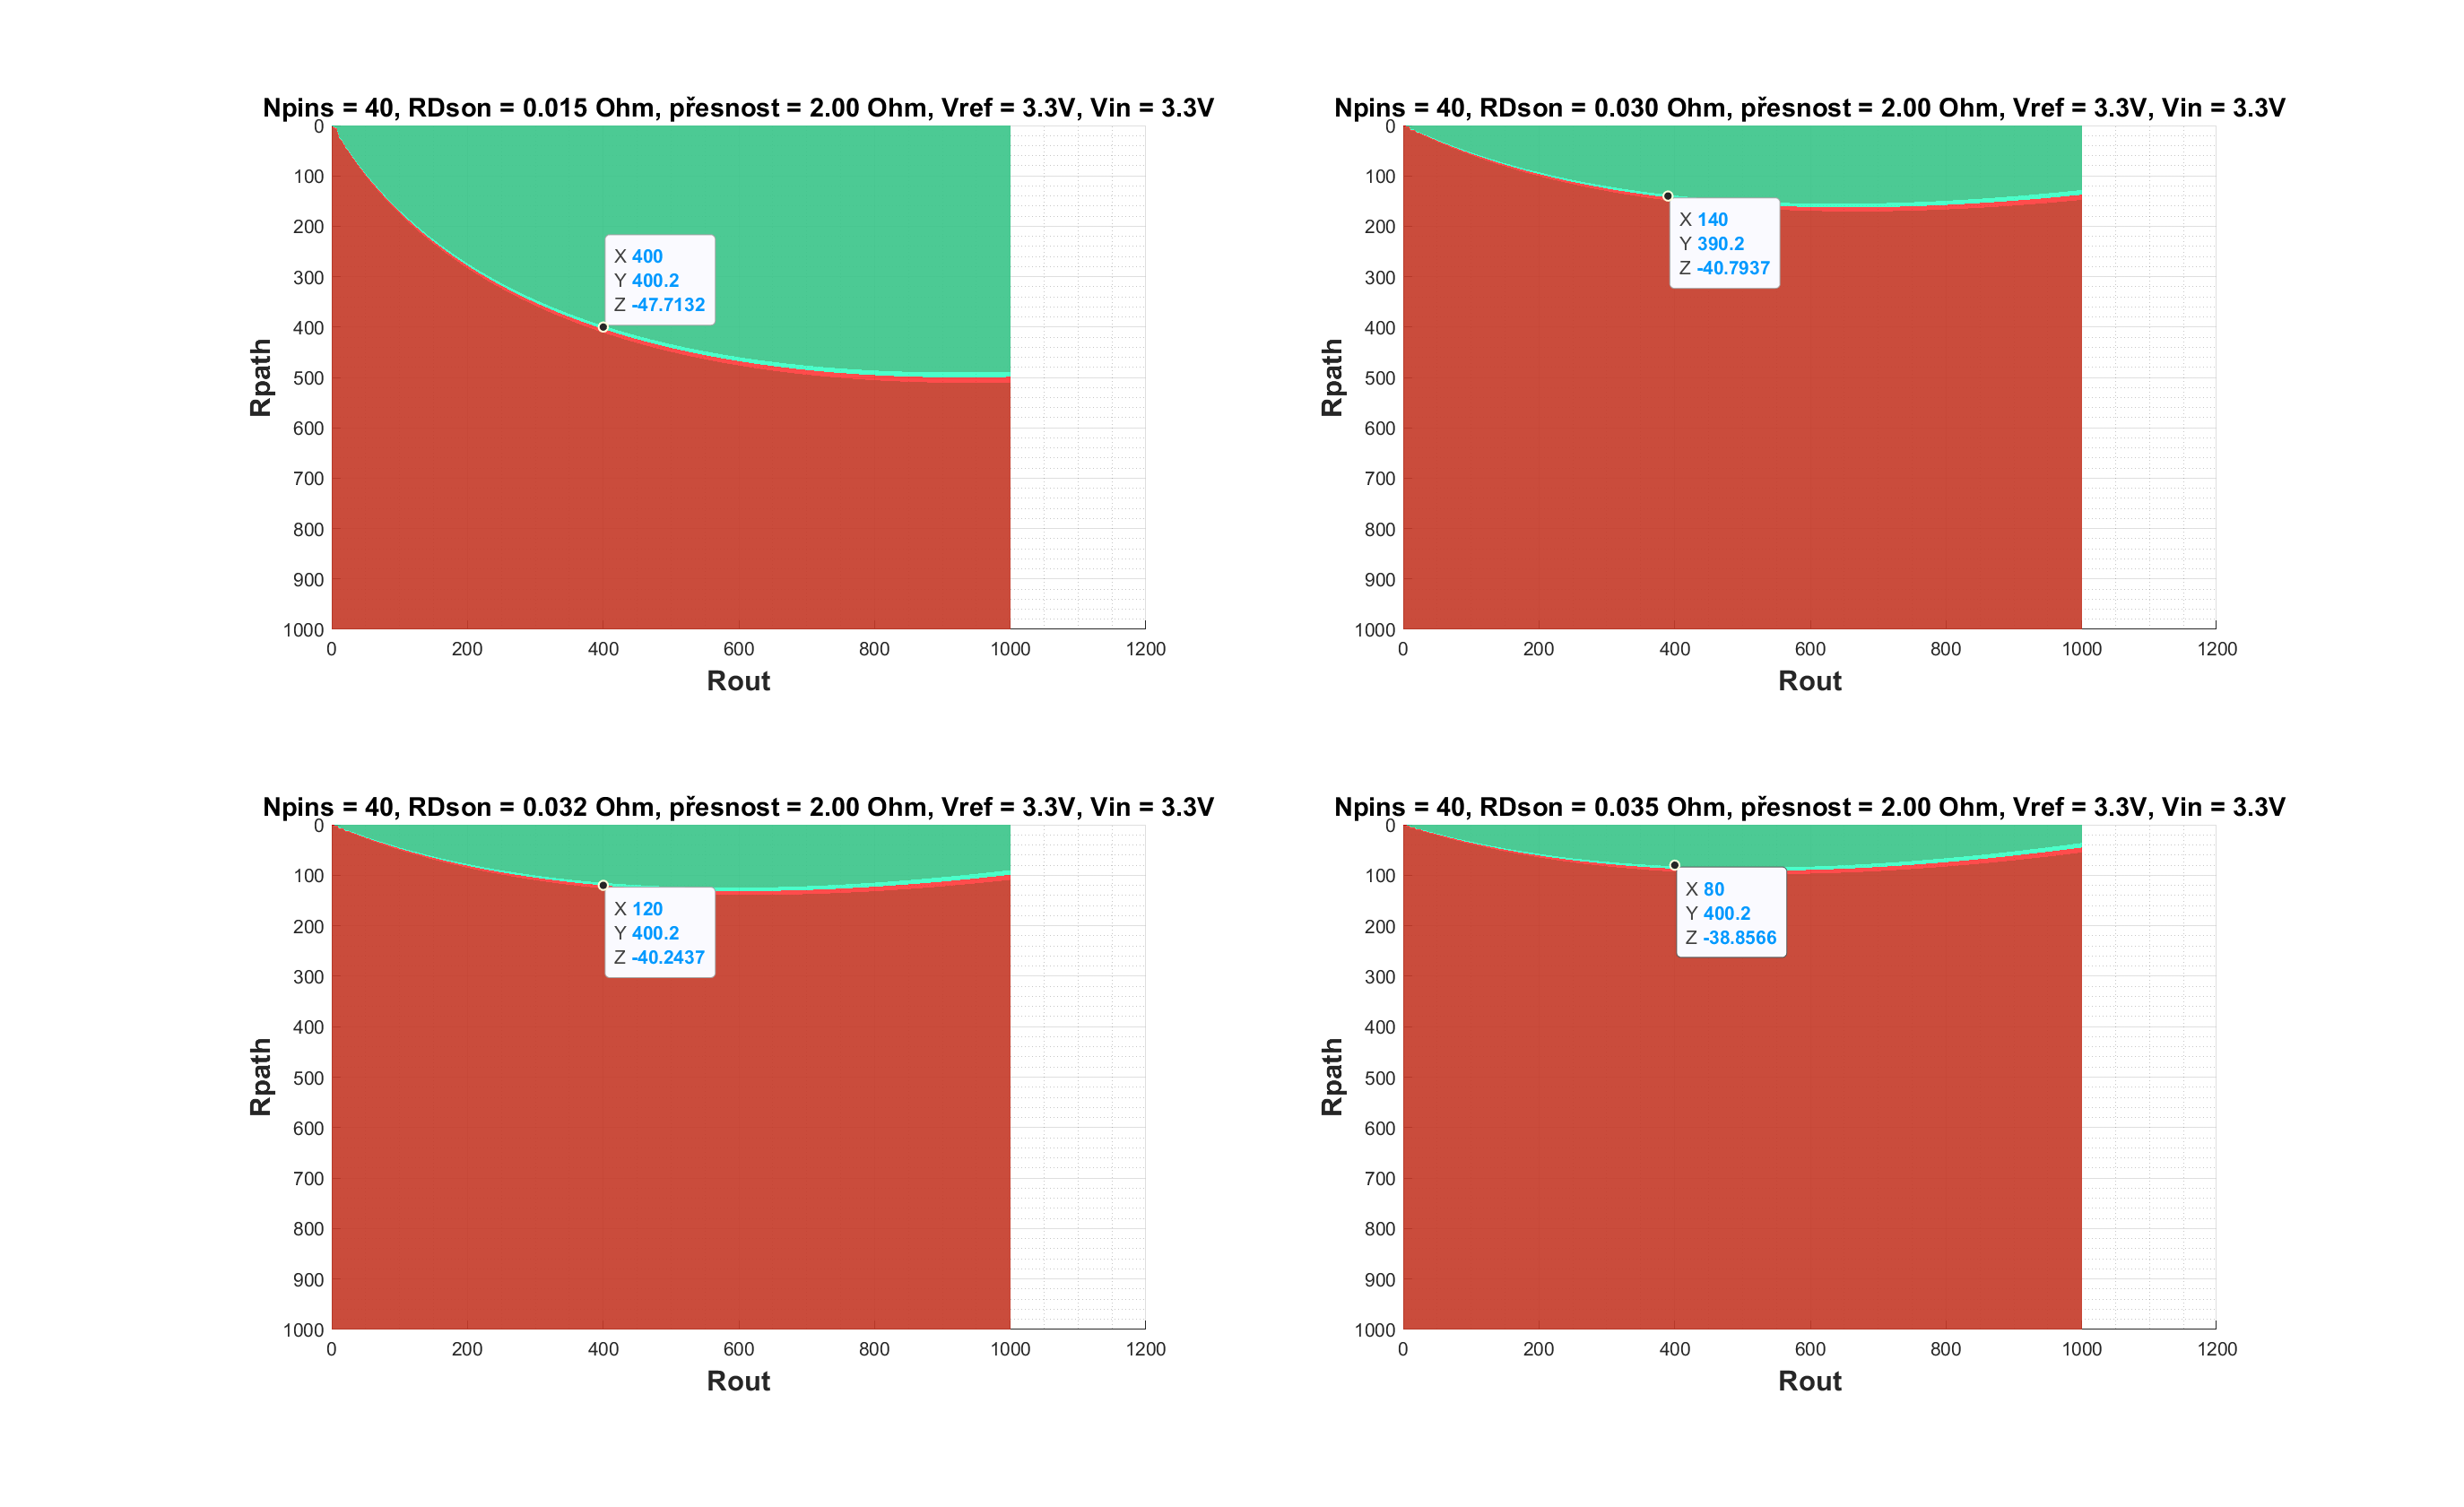
\includegraphics[width = 1\textwidth]{obrazky/vliv_RDSON.eps}
    \caption{vliv RDSon na přesnost měření (generováno pomocí MATLAB)}
    \label{fig:vliv RDSon}
\end{figure}

Na základě výše zmíněným požadavků byl zvolen mosfet SSM3J358R,LF. Níže je výstřižek z datasheetu. Podle typických hodnot by se mělo
docílit $R_{DSon}$ do 25\,m$\Omega$.
\begin{figure}[ht!]
    \centering
    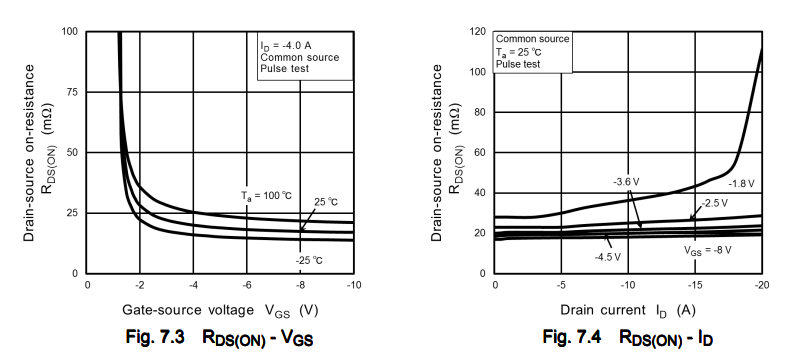
\includegraphics[height = 0.15\textheight]{obrazky/mosfet_datasheet.png}
    \caption{Výstřižek z datasheetu mosfetu SSM3J358R,LF - RDSON\cite{PMOS_datasheet}}
    \label{fig:Výstřižek z datasheetu mosfetu SSM3J358R,LF - RDSON}
\end{figure}

\clearpage

\subsubsection{Volba N-channel mosfetu}
Parametry N-channel mosfetu nemají příliš velký vliv na chování obvodu, protože jeho odpor $R^N_{DSon}$ je započítán do hodnoty odporu $R_{out}$.
Zároveň je hodnota $R^N_{DSon}$ většinou nižší než tolerance odporu $R_{out}$. Hlavním požadavkem je zde, aby bylo možno ovládat mosfet 3.3 a 5V logikou.
Dále by měl mosfet být schopen snést proud I = 3.3/400 = 8.25mA, byl co nejlevnější dostupný a měl menší velikost pouzdra. Byl vybrán PJA3432\_R1\_00001
s následujícími parametry.\\

\begin{figure}[ht!]
    \centering
    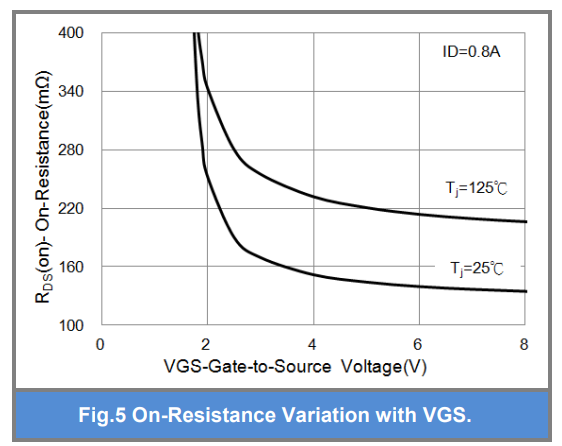
\includegraphics[height = 0.25\textheight]{obrazky/Nmosfet_datasheet.png}
    \caption{Výstřižek z datasheetu N-channel mosfetu PJA3432\_R1\_00001 - RDSON\cite{NMOS_datasheet}}
    \label{fig:Výstřižek z datasheetu N-channel mosfetu}
\end{figure}

\subsubsection{Volba komparátoru}
Doposud nebylo počítáno s vlivem reálného komparátoru.
Aby byly výsledky co nejpřesnější je vhodné zvolit komparátor s co nejvyšším vstupním odporem.
Protože při propojení pinů nízkou hodnotou odporu je výstupní napětí děliče blízké napájecímu napětí, tak je komparátor
napájen vyšším napájecím napětím konfigurovatelným od cca 4 do 5.5V (více v sekci o napájení).
Komparátor by také neměl mít hysterzi. Dále, protože je vstup komparátoru přímo připojen
na bRC piny, tak by zde měla být ESD ochrana.\\

Pro jednodušší PCB layout je vhodné, aby pouzdro obsahovalo více komparátorů.
Co se týče input voltage offsetu, tak na jeho velikosti
příliš nezáleží, protože bude minimalizován kalibrací. Offset by však měl být stabilní.\\

Byl vybrán komparátor LM393LVQDRQ1. Vstup komparátoru je interně chráněn proti ESD do 2kV.
Na výstupu komparátoru je pull-up rezistor připnutý k napájení
ovládací karty (tímto je docíleno napěťové kompatibility s 3V3 i 5V logikou).
Vybraný komparátor má poměrně vysokou kapacitu vstupu (3\,pF).
Vliv kapacity je diskutován v sekci o návrhu D/A převodníku ovládací karty\cite{comp_datasheet}.


\subsubsection{Volba shift registrů}
Základním požadavkem na shift registry je možnost řízení pomocí 3V3 logiky, přičemž shift registr samotný je napájen 5V.
Dále schopnost řídit vybrané P a N-Channel mosfety. Všech 80 výstupů (P-Mosfetů) je řízeno 2x5 shift registry zapojených do série.
Pro výstupní piny není kladen velký důraz na rychlost nastavení hodnot,
protože pro každý výstupní pin je nutné změřit dalších 4000 vstupních tak je na přepínání času dostatek.
Naopak ovládání N-channel mosfetů by mělo být co nejrychlejší.\\

V kapitole o výběru rezistoru děliče je zmíněno, že bude možné měřit 40 pinů současně.
Jistým kompromisem jednoduchosti ovládání a rychlostí je tak ovládat N-channel mosfety 10 shift
registry zapojenými stylem 2x5 do série (viz. schéma měřící karty v příloze).\\

Toto řešení ovládání je zároveň modulární, lze odebírat celé bloky po 8 pinech a
zlevnit tak měřící kartu pro použití v jednodušších aplikacích. Stejně jako u předchozích součástek i zde
je požadavek na menší pouzdro. Byl vybrán shift registr SN74AHCT595PWR.
Tento shift registr je 3 stavový, lze tak přímo řídit jednotlivé mosfety bez nutnosti
pull-up/down rezistorů. Poblíž napájení každého z shift registrů je umístěn 100nF vazební kondenzátor.
Řídící piny shift registrů jsou přivedeny na 2x25 pinový konektor,
kterým je měřící deska připojena k ovládací desce\cite{shift_datasheet}.

\subsubsection{Volba multiplexerů}
Multiplexer by měl být ovladatelný 3.3V i 5V logikou. Byl zvolen multiplexer\\ TMUX1308QDYYRQ1.
K multiplexeru je obdobně jako k shift registru připojen 100nF vazební kondenzátor.
Komparátory jsou zapojeny stylem 2x5 a mají jednotnou adresaci (2x3 adresní piny, 2x enable pin, 2x5 výstupních pinů).
Výstupy multiplexeru jsou přivedeny na 2x25 pinový konektor\cite{mux_datasheet}.

\clearpage

\subsection{Napájecí část}
Měřící karta je ve svém
standardním provedení napájena 7V až 15V.
Toto napájecí napětí je následně regulováno
dvěma nastavitelnými regulátory TLV76701DGNR na 3V a 5V .
Tyto regulátory disponují enable pinem, kterým je možné spínat regulátory ve správném pořadí,
tak aby nedocházelo k nedefinovaným stavům. Enable piny jsou řízeny pomocí ovládací karty, je však možno
pomocí jumperů přepnout regulátory do režimu, kde se spínají současně automaticky.
Dále tyto regulátory nabízí výstupní proud až 1A, ESD ochranu vstupů a automatickou tepelnou ochranu.\cite{regulator_datasheet}\\

\begin{figure}[ht!]
    \centering
    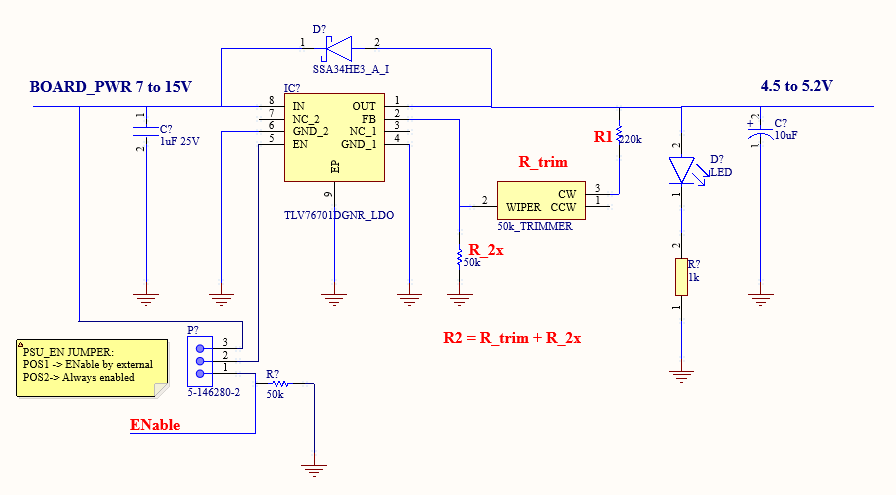
\includegraphics[width = 1\textwidth]{obrazky/PSU.png}
    \caption{Napájení měřící karty: 5V regulátor (celé schéma měřící karty v příloze -  POWER REGULATORS)}
    \label{Napájení měřící karty: 5V regulátor}
\end{figure}

Napětí 5V, ve finálním schématu v příloze označeno jako Vcomp,
slouží k napájení multiplexerů, komparátorů a shift registrů. Ve zpětnovazebním obvodu regulátoru
je připojen odporový dělič s 50\,k$\Omega$ trimmerem, pomocí kterého lze nastavit výstupní napětí v rozmezí
přibližně od 4.5 do 5.2V. Vzhledem k povaze napájených komponentů se nepředpokládá vysoký odběr proudu.\\

Napětí 3V, ve finálním schématu v příloze označeno jako Vpins, slouží k generování napětí na bRC pinech. Obdobně jako regulátor pro 5V má i regulátor pro 3V trimmer pro
nastavení výstupního napětí. Zde je však v napěťovém děliči zvolena jiná hodnota pevného rezistoru R1, tak aby
bylo možno pomocí 50\,k$\Omega$ trimmeru nastavit výstupní napětí v rozmezí od 2.8 do 3.5V.
Protože bude referenční napětí generováno 3.3V D/A převodníkem. Počítá se s nastavením výstupního napětí na 3V pro 
případ, že by převodník nefungoval v celém svém rozsahu. 3V regulátor musí být schopen dodat do obvodu proud minimálně
330mA (zdůvodnění je patrné z rovnice \ref{eq:MIN_CURRENT}).
Volba hodnot rezistorů ve zpětné vazbě vychází z rovnice pro výstupní napětí regulátoru
\begin{equation}
    V_{out} = V_{FB}  \cdot (1 + \frac{R1}{R2}),
\end{equation}

\noindent kde $V_{FB}$ = 0.8V, pro R2 byl použit 50\,k$\Omega$ trimmer v sérii s odporem 50\,k$\Omega$.
Hodnota R1 pro 5V regulátor byla zvolena
220\,k$\Omega$ a pro 3V regulátor 120\,k$\Omega$.\\

Regulátory mají připojeny shotky diody SSA34HE3. Tyto diody slouží jako ochrana proti přepětí na výstupu.
Na výstupu regulátorů jsou připojeny LED pro snadnou kontrolu, zda je regulátor zapnutý.
Výstupy regulátorů jsou přivedeny na jak na 2x25 pin konektor, tak na pole pinů pro připojení bRC (případně DIN konektoru).
Je tak možno využít výstupní napětí regulátorů pro napájení externích komponent, nebo
také regulátory neosazovat a napájet měřící kartu externím regulovaným zdrojem.\\

Na měřící kartě lze také nalézt napětí, které je ve finálním schématu v příloze označeno jako PWR\_MCU.
Toto napětí je do měřící desky přivedeno z ovládací karty. Je to napětí, které je následně využito
pro výstup multiplexerů (pull up výstupu komparátoru) a je tím zajištěna napěťová kompatibilita s ovládací logikou 3.3V a 5V.


\subsection{Návrh PCB}
Pro návrh PCB bylo využito softwaru Altium Designer. PCB bylo vyrobeno firmou
JLCPCB.
Jedná se o 6-ti vrstvé PCB s následujícím rozložením vrstev.
Jednotlivé vrstvy mají následující účel:
\begin{itemize}
    \item TOP layer: signal; polygon - GND
    \item inner layer 1: GND
    \item inner layer 2: signal; polygon - GND
    \item inner layer 3: signal/PWR; polygon - PWR\_MCU, Vref
    \item inner layer 4: PWR; polygon - BOARD\_PWR, Vpins, Vcomp
    \item BOTTOM layer: signal; polygon - GND, Vref
\end{itemize}

\noindent Za označením "polygon -"\ jsou uvedeny jména signálů, které mají v dané vrstvě nějaký polygon.
Následující obrázek zobrazuje všechny vrstvy současně bez polygonů. Na další straně jsou jednotlivé vrstvy
včetně polygonů.

\begin{figure}[ht!]
    \centering
    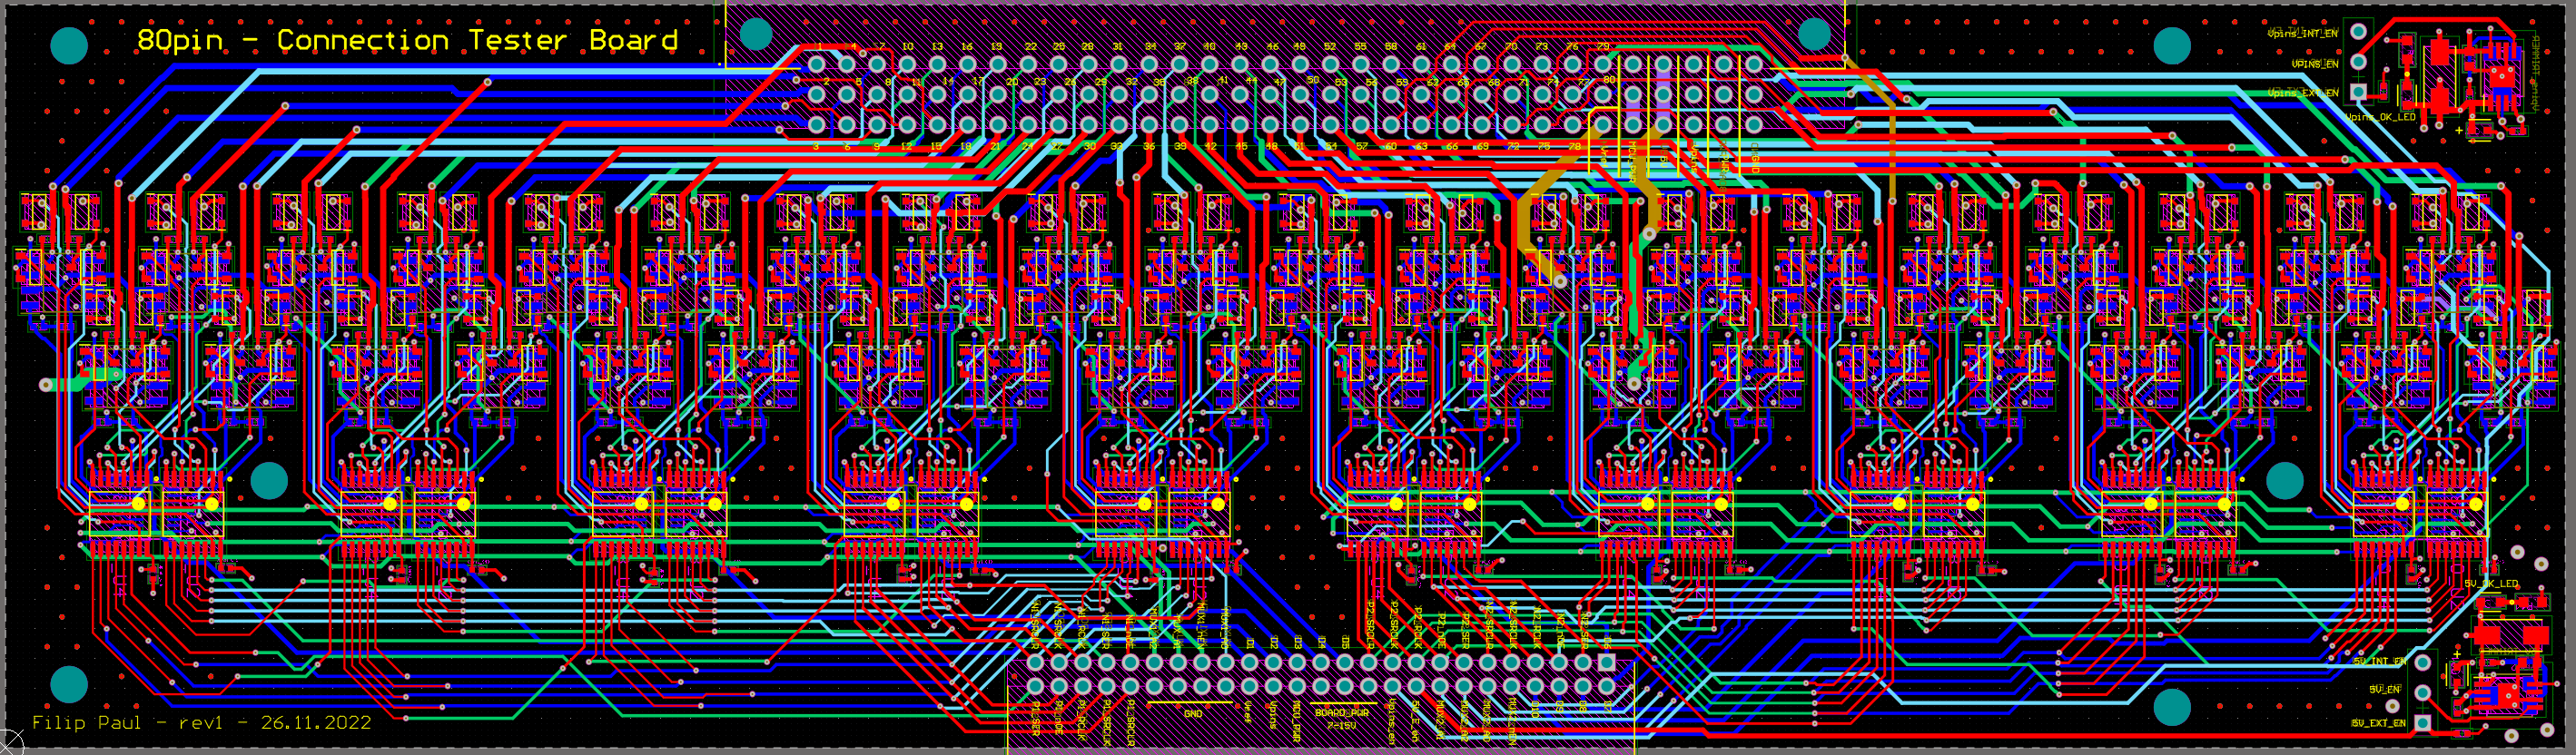
\includegraphics[width = 1\textwidth]{obrazky/all_layers_no_poly.png}
    \caption{Všechny vrstvy bez polygonů}
    \label{fig:Všechny vrstvy bez polygonů}
\end{figure}
\clearpage

\begin{figure}[ht!]
    \centering
    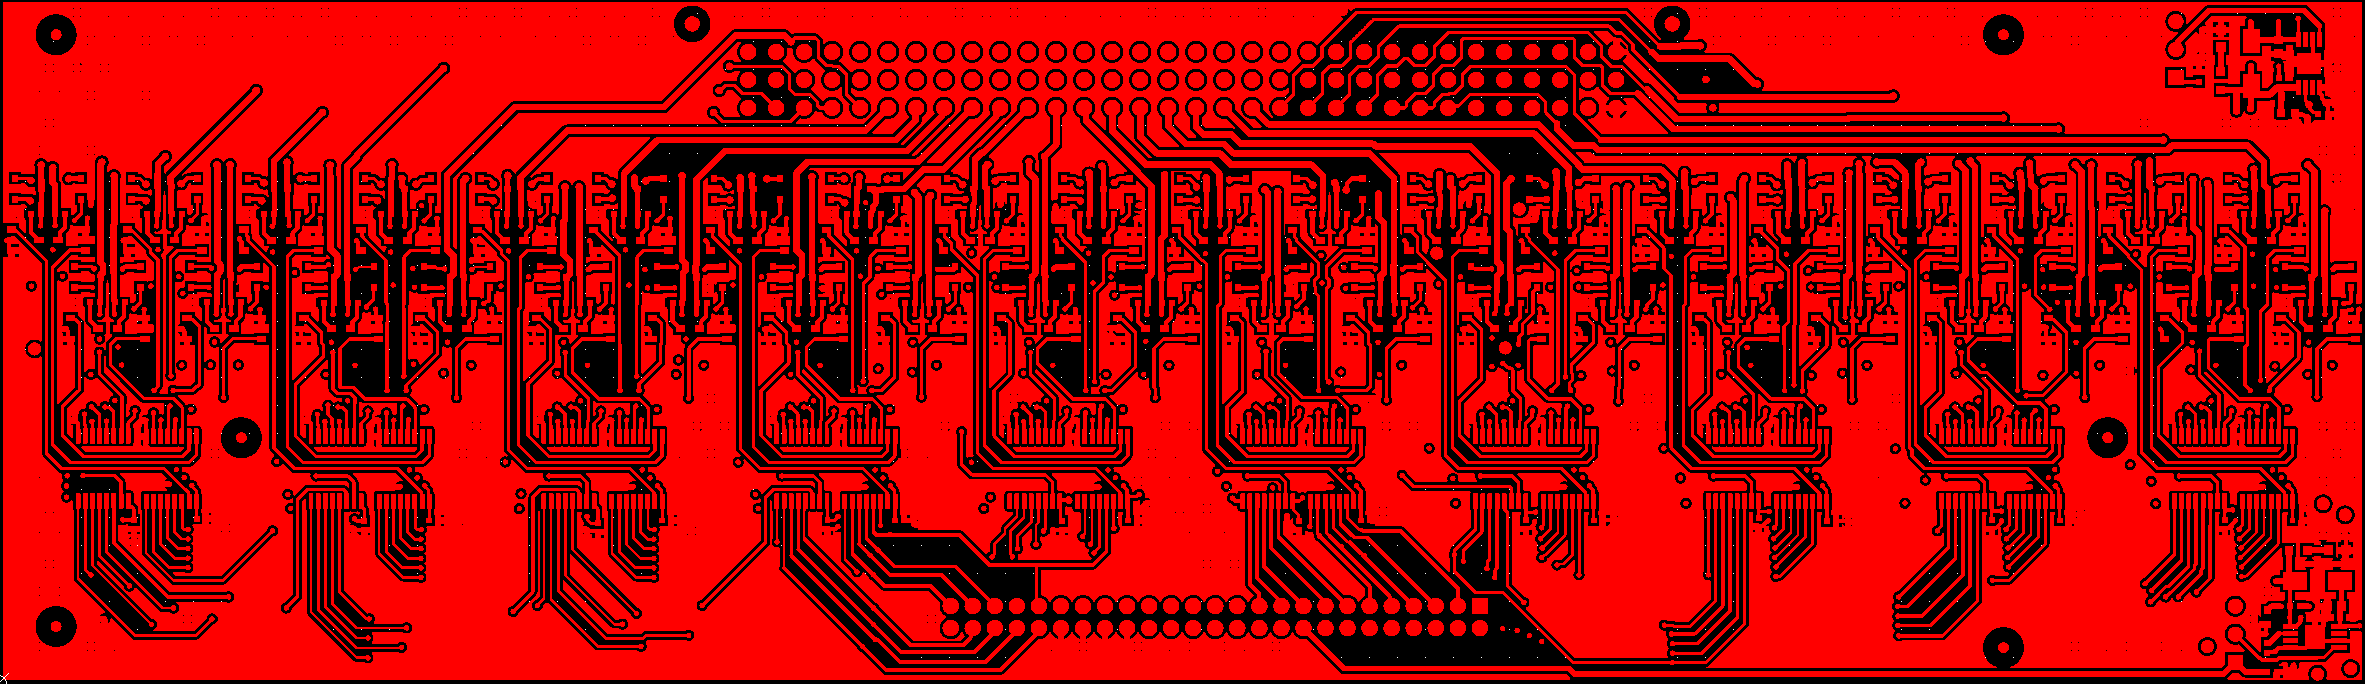
\includegraphics[height = 0.15\textheight]{obrazky/layer_top.png}
    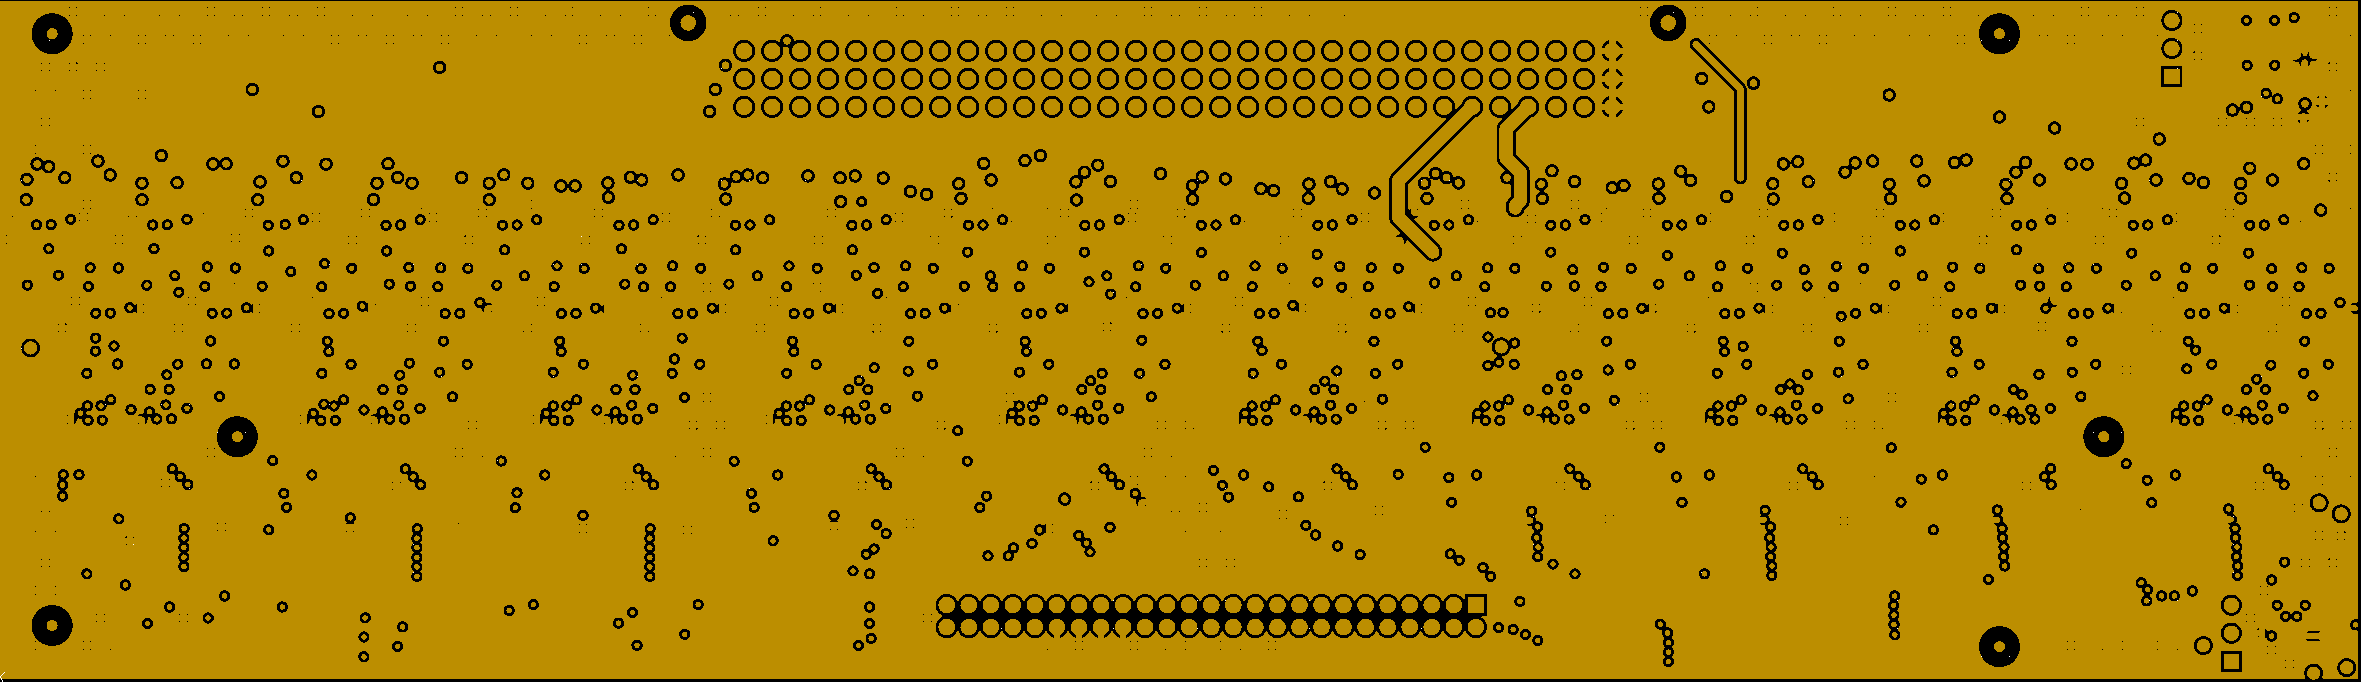
\includegraphics[height = 0.15\textheight]{obrazky/layer_2.png}
    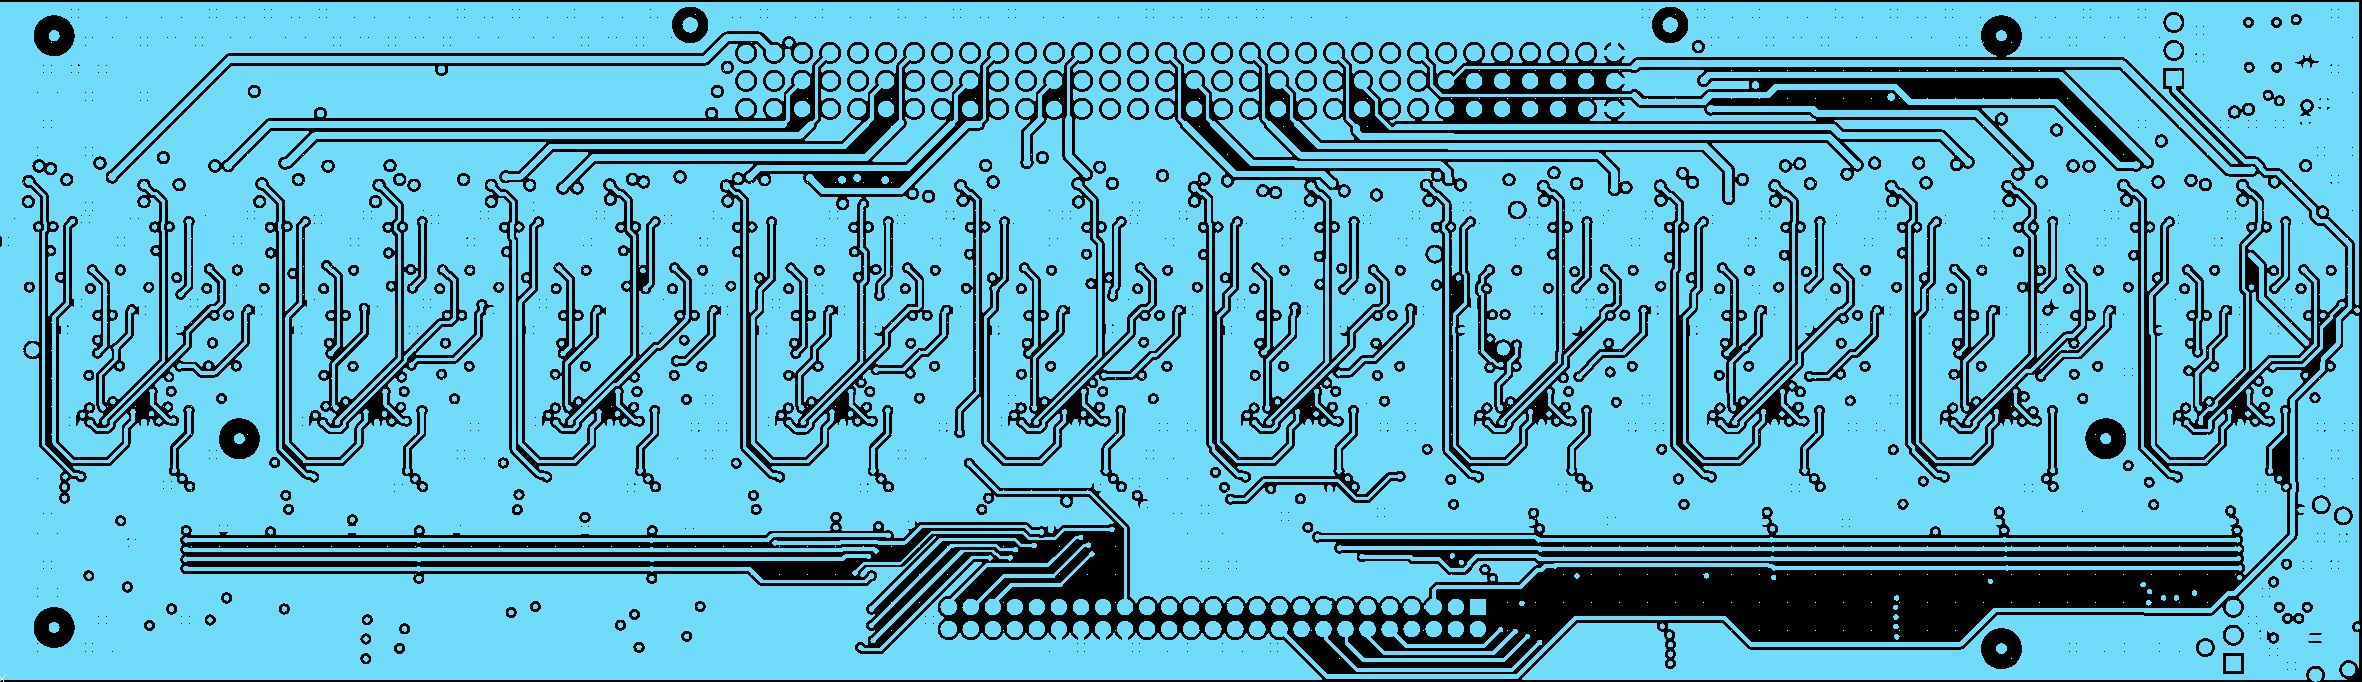
\includegraphics[height = 0.15\textheight]{obrazky/layer_3.png}
    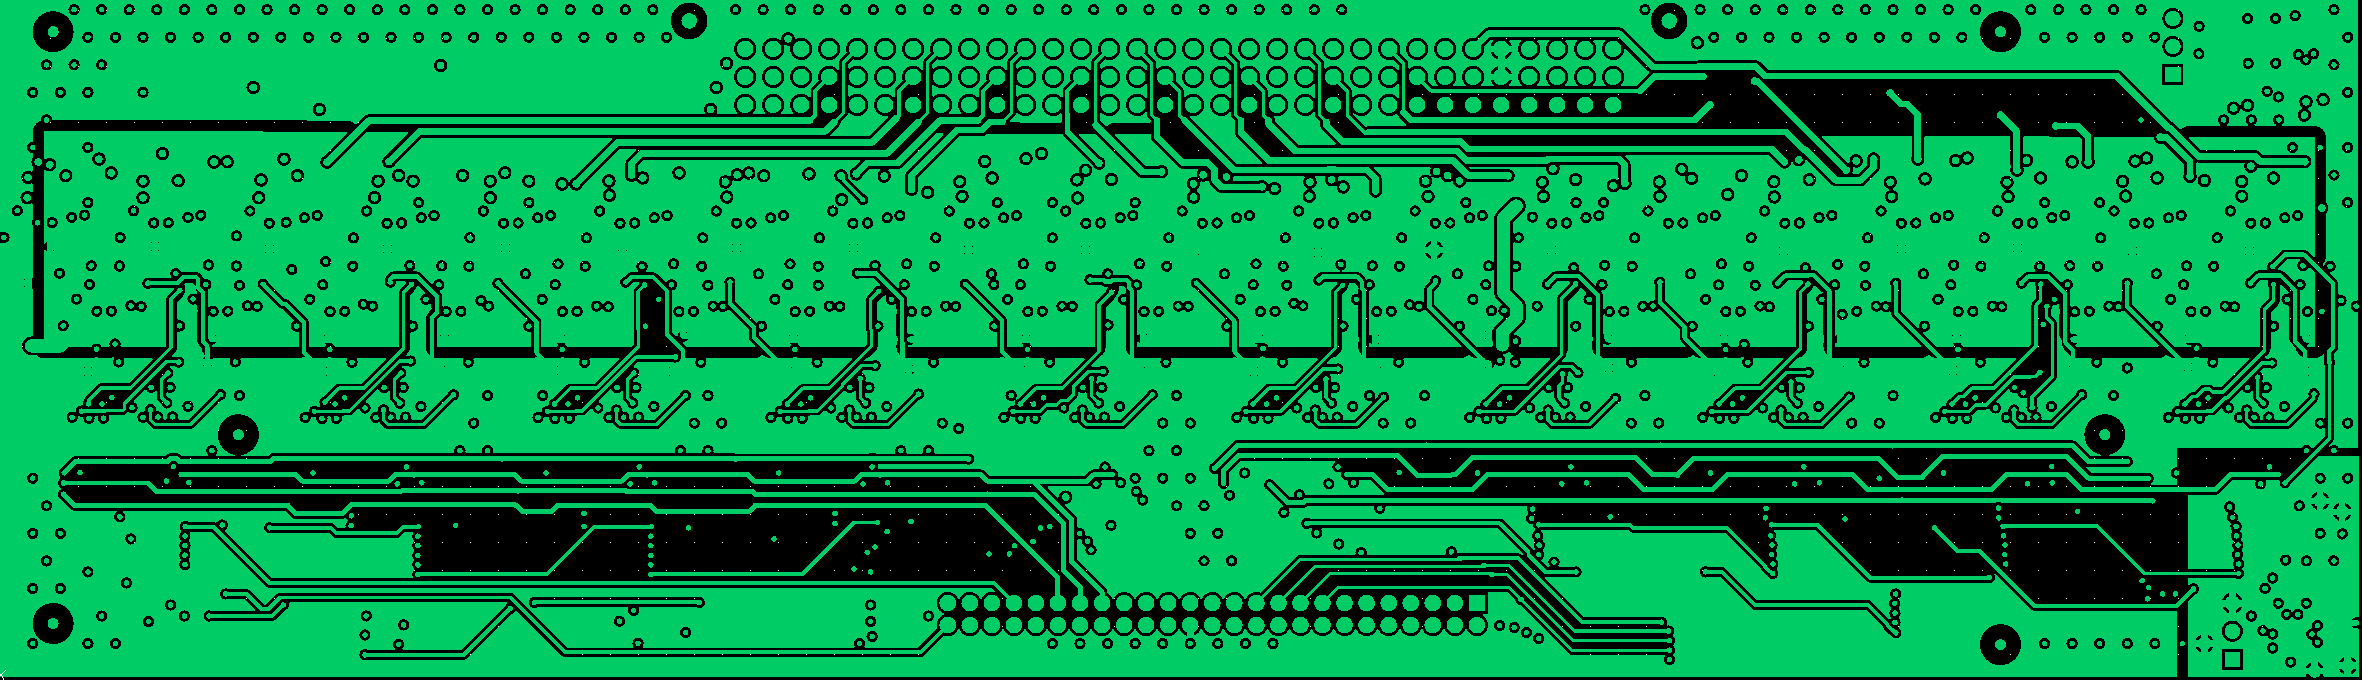
\includegraphics[height = 0.15\textheight]{obrazky/layer_4.png}
    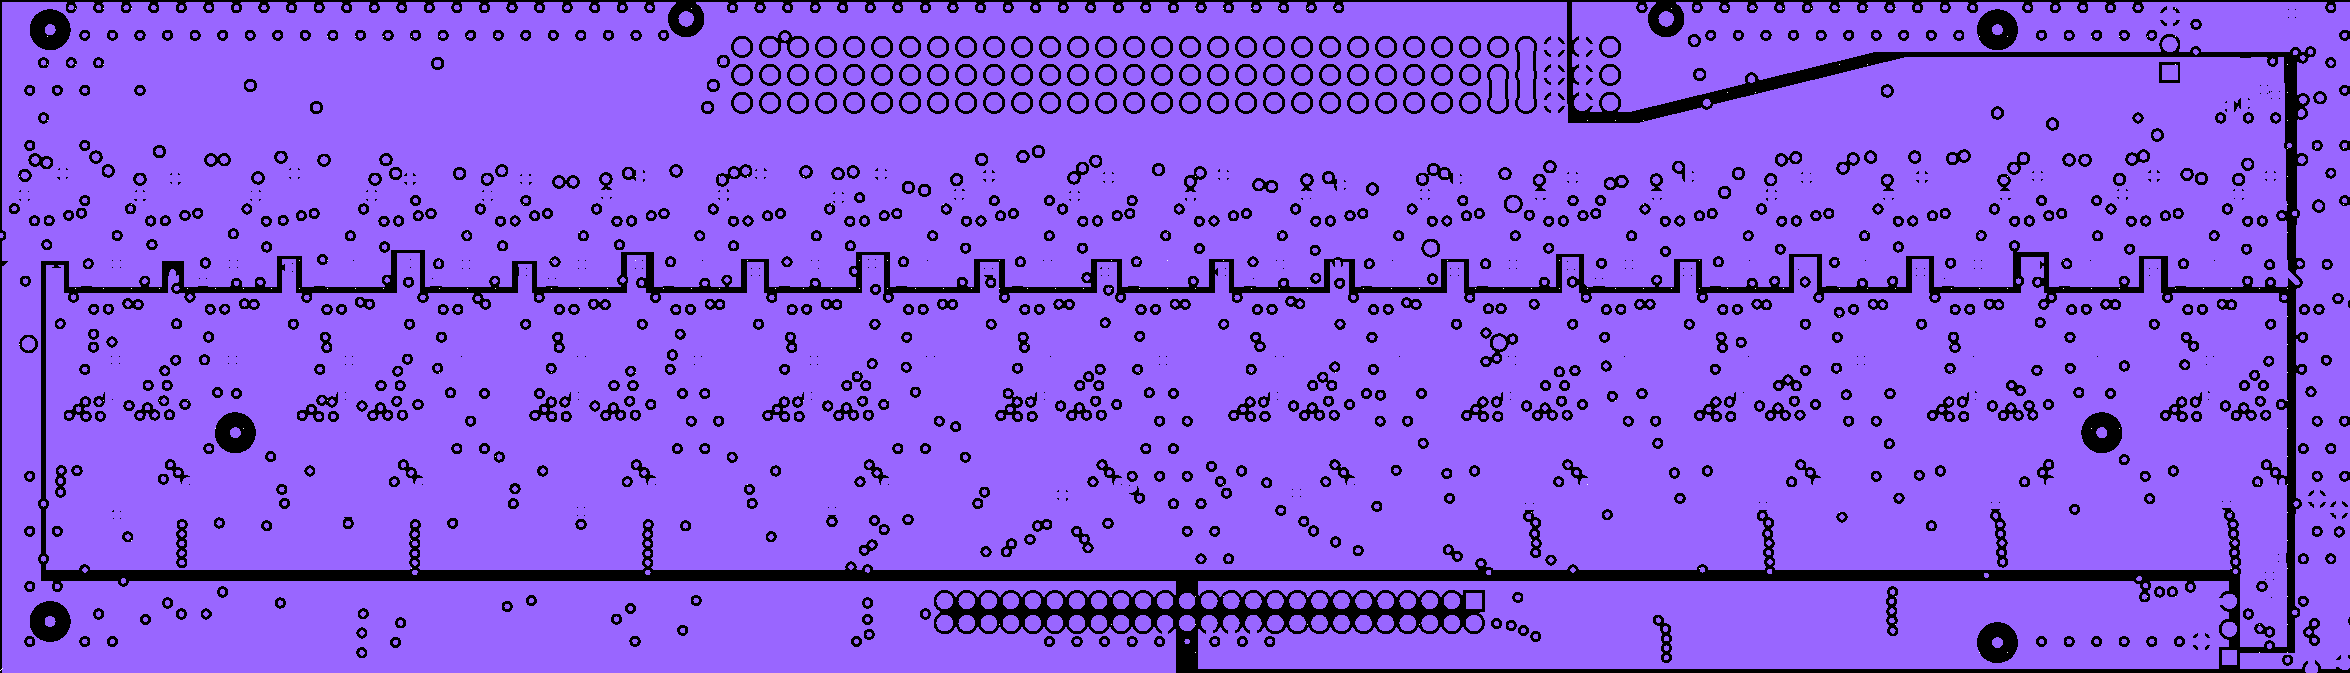
\includegraphics[height = 0.15\textheight]{obrazky/layer_5.png}
    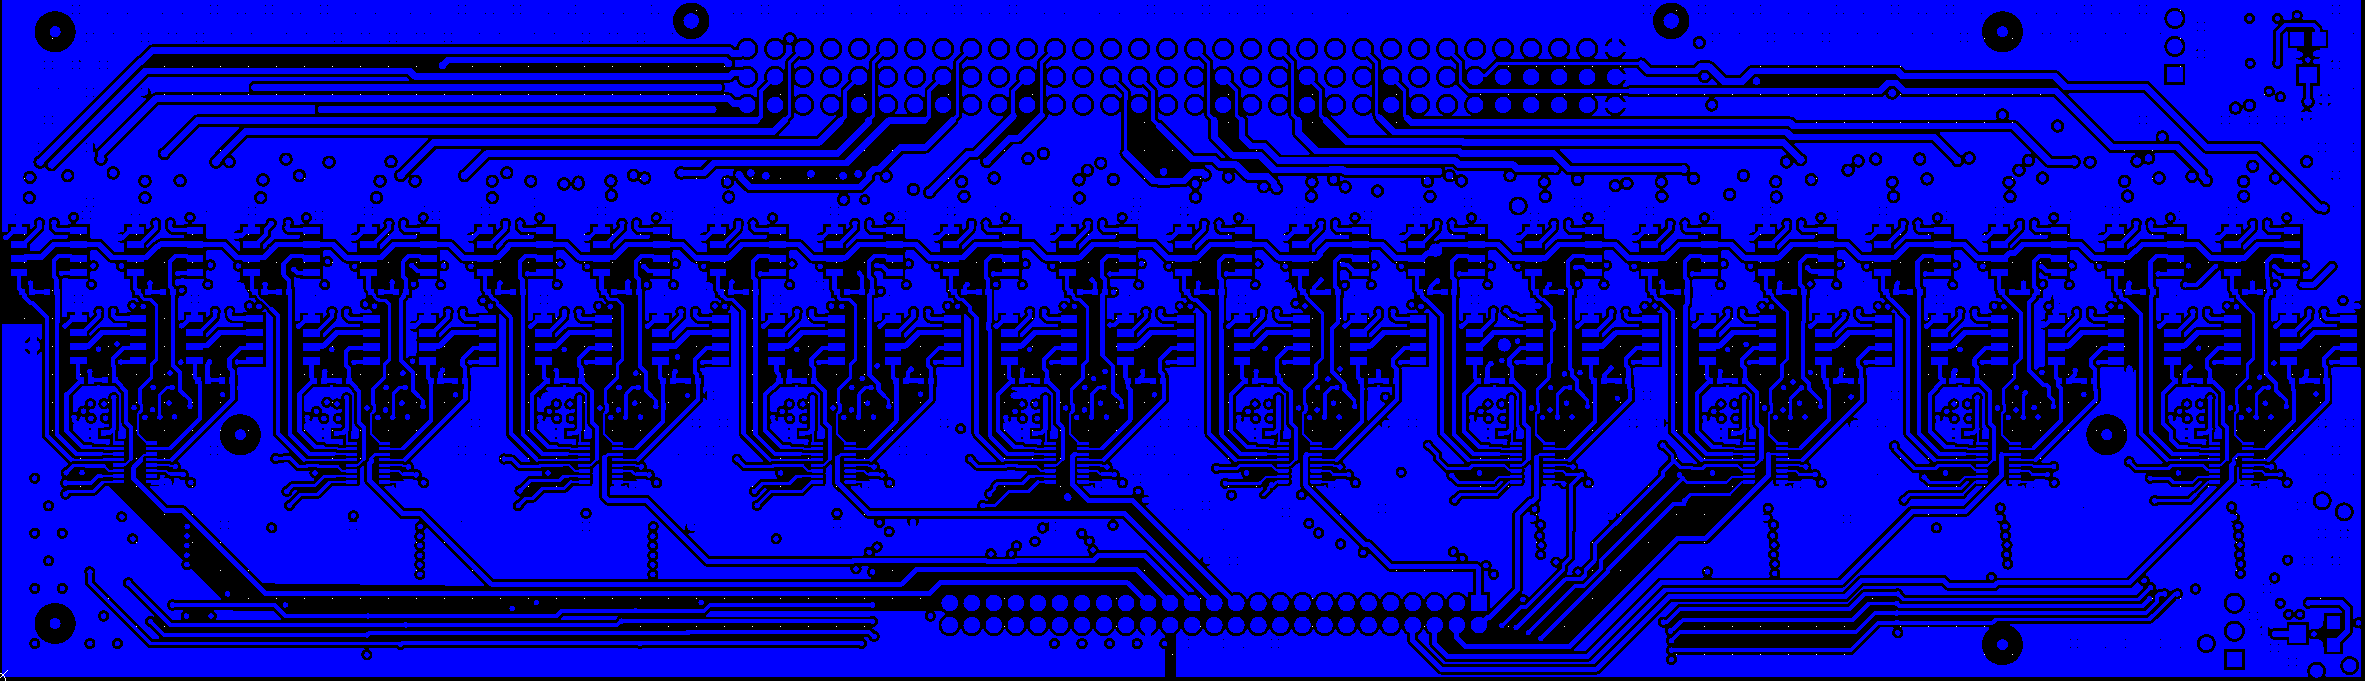
\includegraphics[height = 0.15\textheight]{obrazky/layer_bot.png}
    \caption{Vrstvy PCB top to bottom včetně polygonů}
    \label{fig:Vrstvy PCB top to bottom}
    
\end{figure}

\clearpage

Pro minimalizaci zemních smyček jsou po celé desce rozmístěny stitching vias,
které propojují GND signály.
V gerber datech a 3D modelu jsou stitching vias zobrazeny jako tented vias. Nicméně kvůli nižší ceně výroby PCB
jsou použity odkryté vias.
Z důvodu požadavků na osazení komponent byl použita použita ENIG povrchová úprava.\\

Důležitou podmínkou návrh PCB měřících karet je, že jejich výška (včetně komponentů) nesmí přesáhnout 8mm.
Tento rozměr je dán roztečí jednotlivých řad bRC pinů. Na následujících obrazcích jsou zobrazeny 3D modely měřící karty
s DIN konektorem, který přesahuje výšku 8mm (nebude však osazen). Finální rozměry měřící karty bez DIN konektoru jsou
(délka x šířka x výška) 215 x 62.5x 7.65mm. PCB obsahuje několik děr pro uchycení pomocí M3 šroubů.


\begin{figure}[ht!]
    \centering
    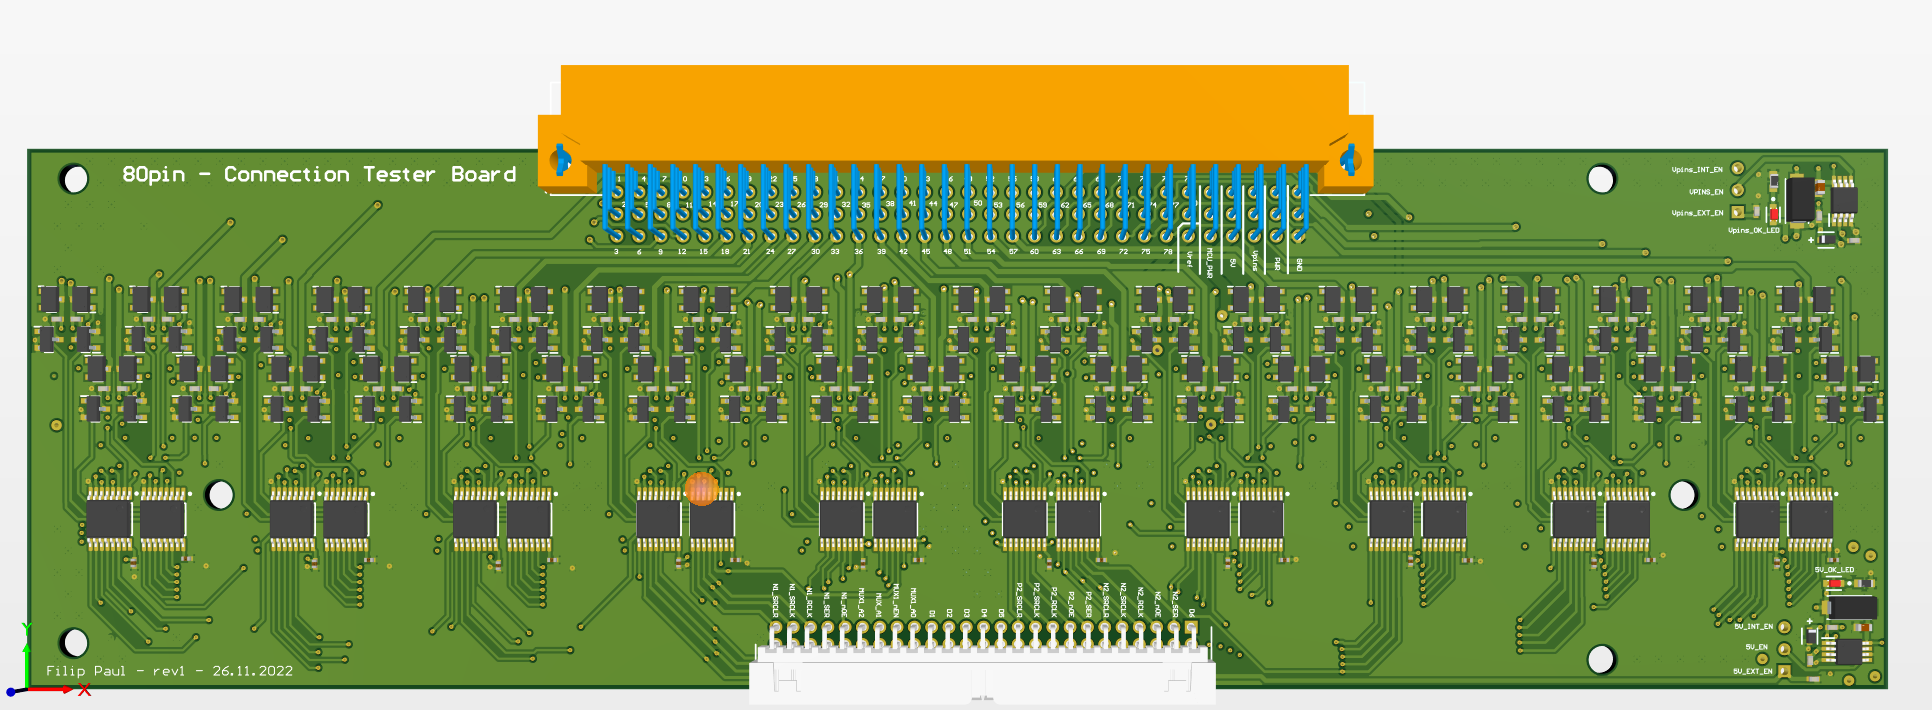
\includegraphics[width = 1\textwidth]{obrazky/karta_3D.png}
    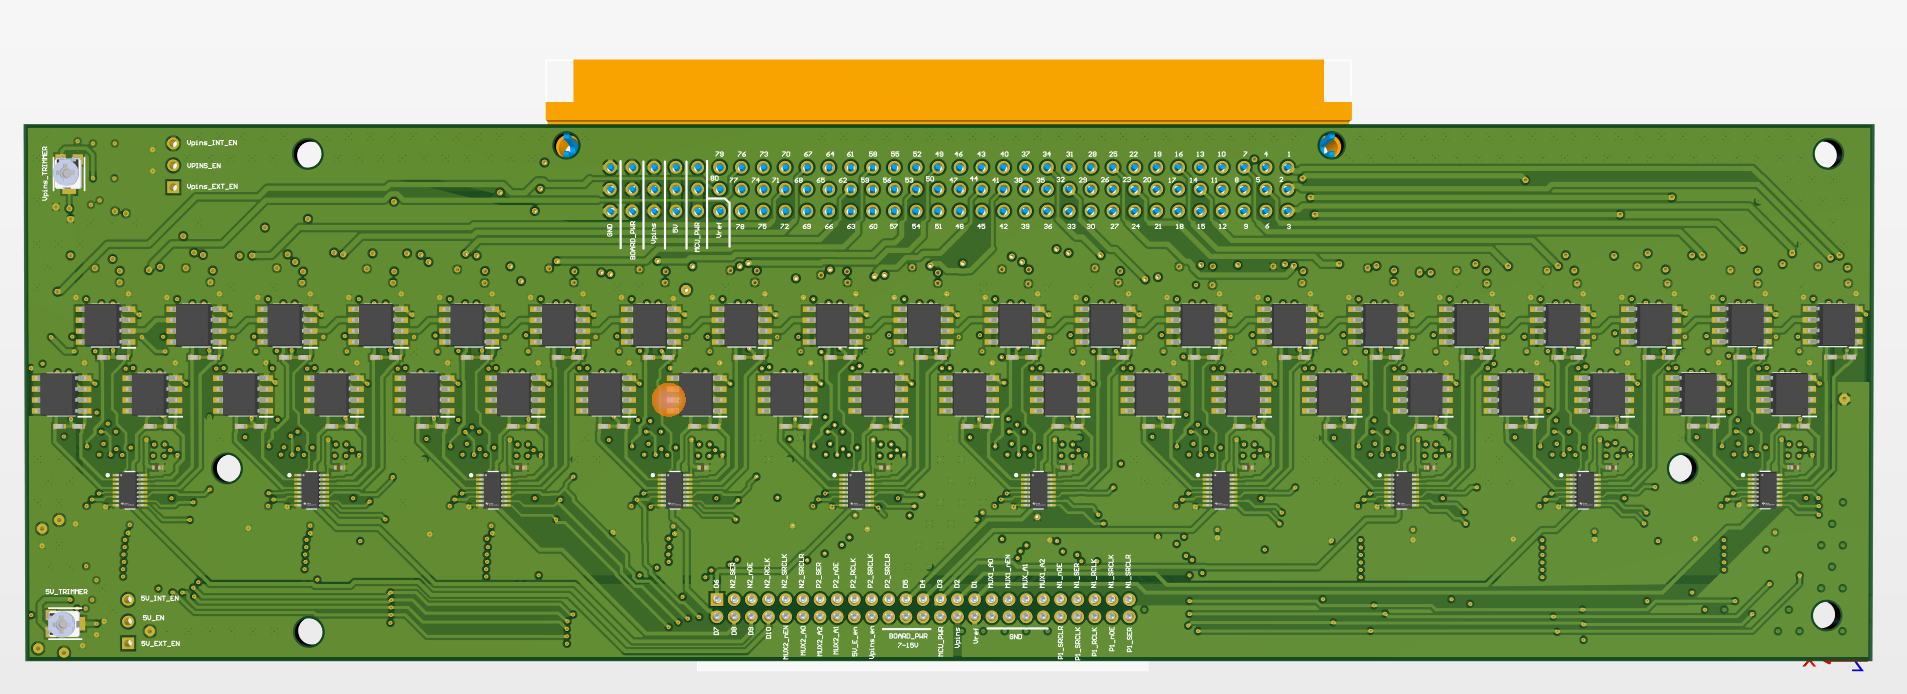
\includegraphics[width = 1\textwidth]{obrazky/karta_3D_bot.png}
    \caption{3D model top a bot s osazeným DIN konektorem}
    \label{fig:3D model top a bot}
    
\end{figure}



